
    \section{SBMOF-1}
    
    \begin{figure}[h!]
       \centering
       \subfigure[]{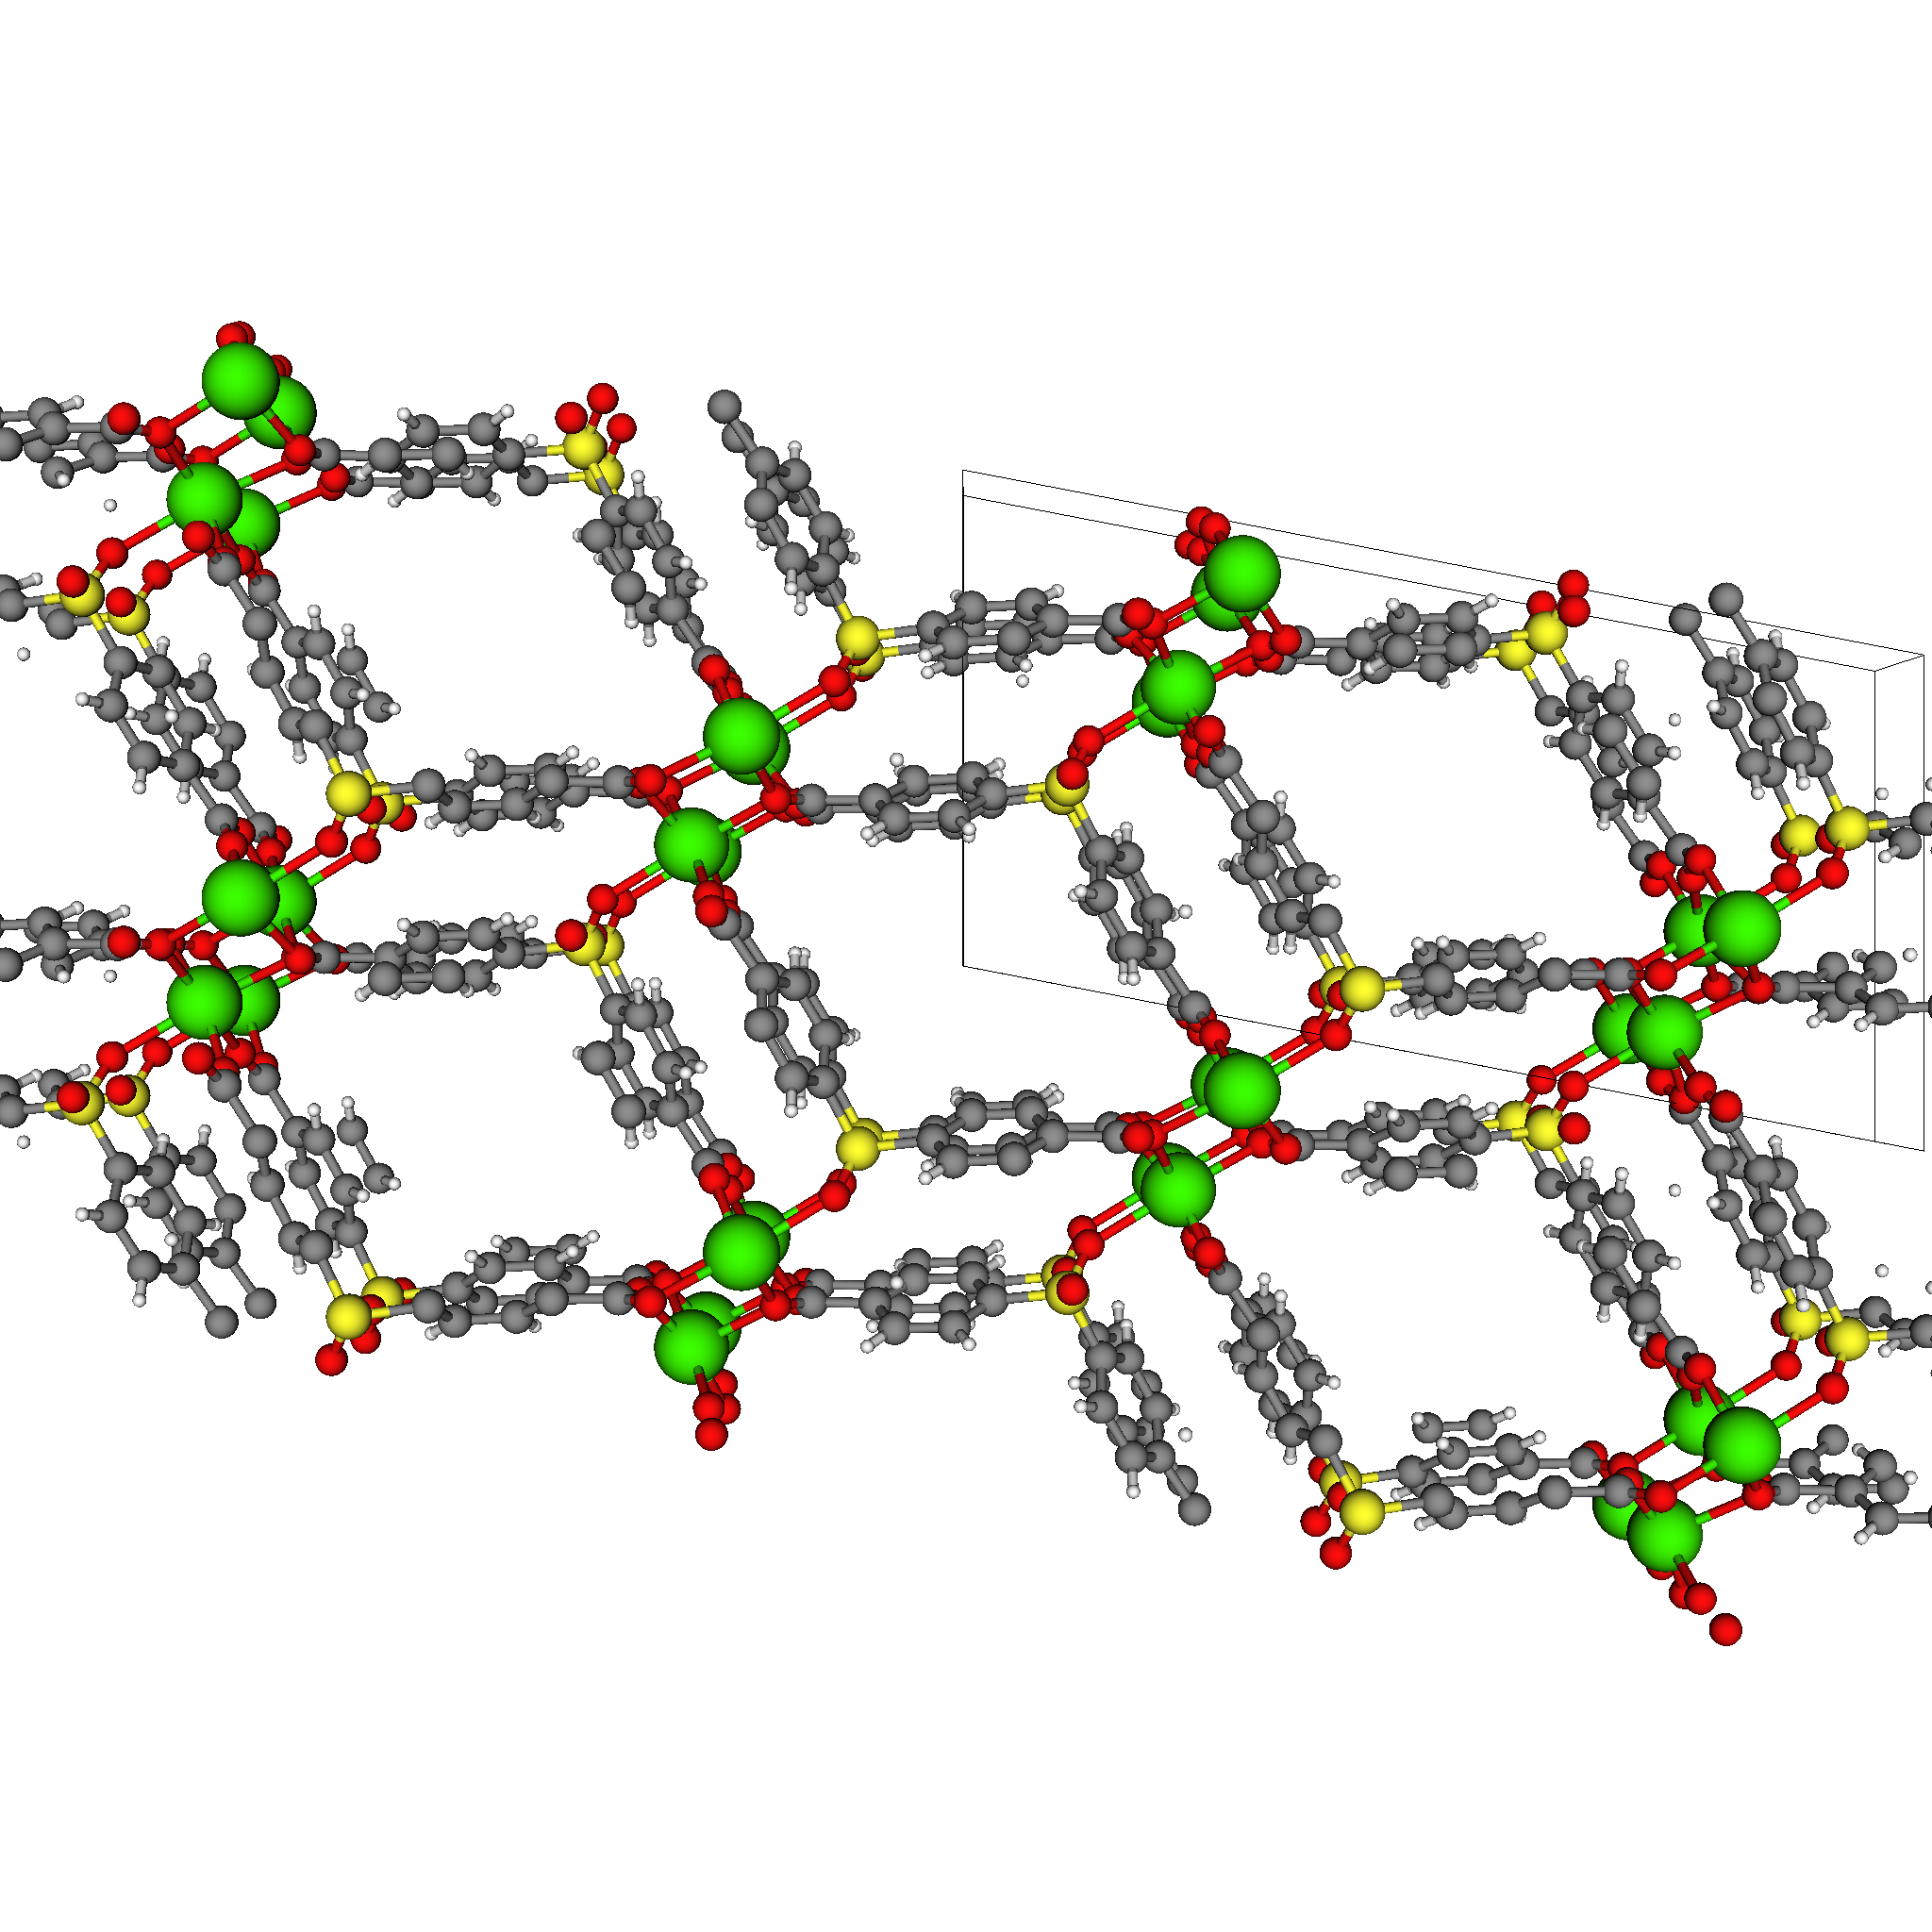
\includegraphics[width=.3\columnwidth]{../xtal_structures/viz/SBMOF-1.png} \label{fig:SBMOF-1_xtal} }
       \subfigure[]{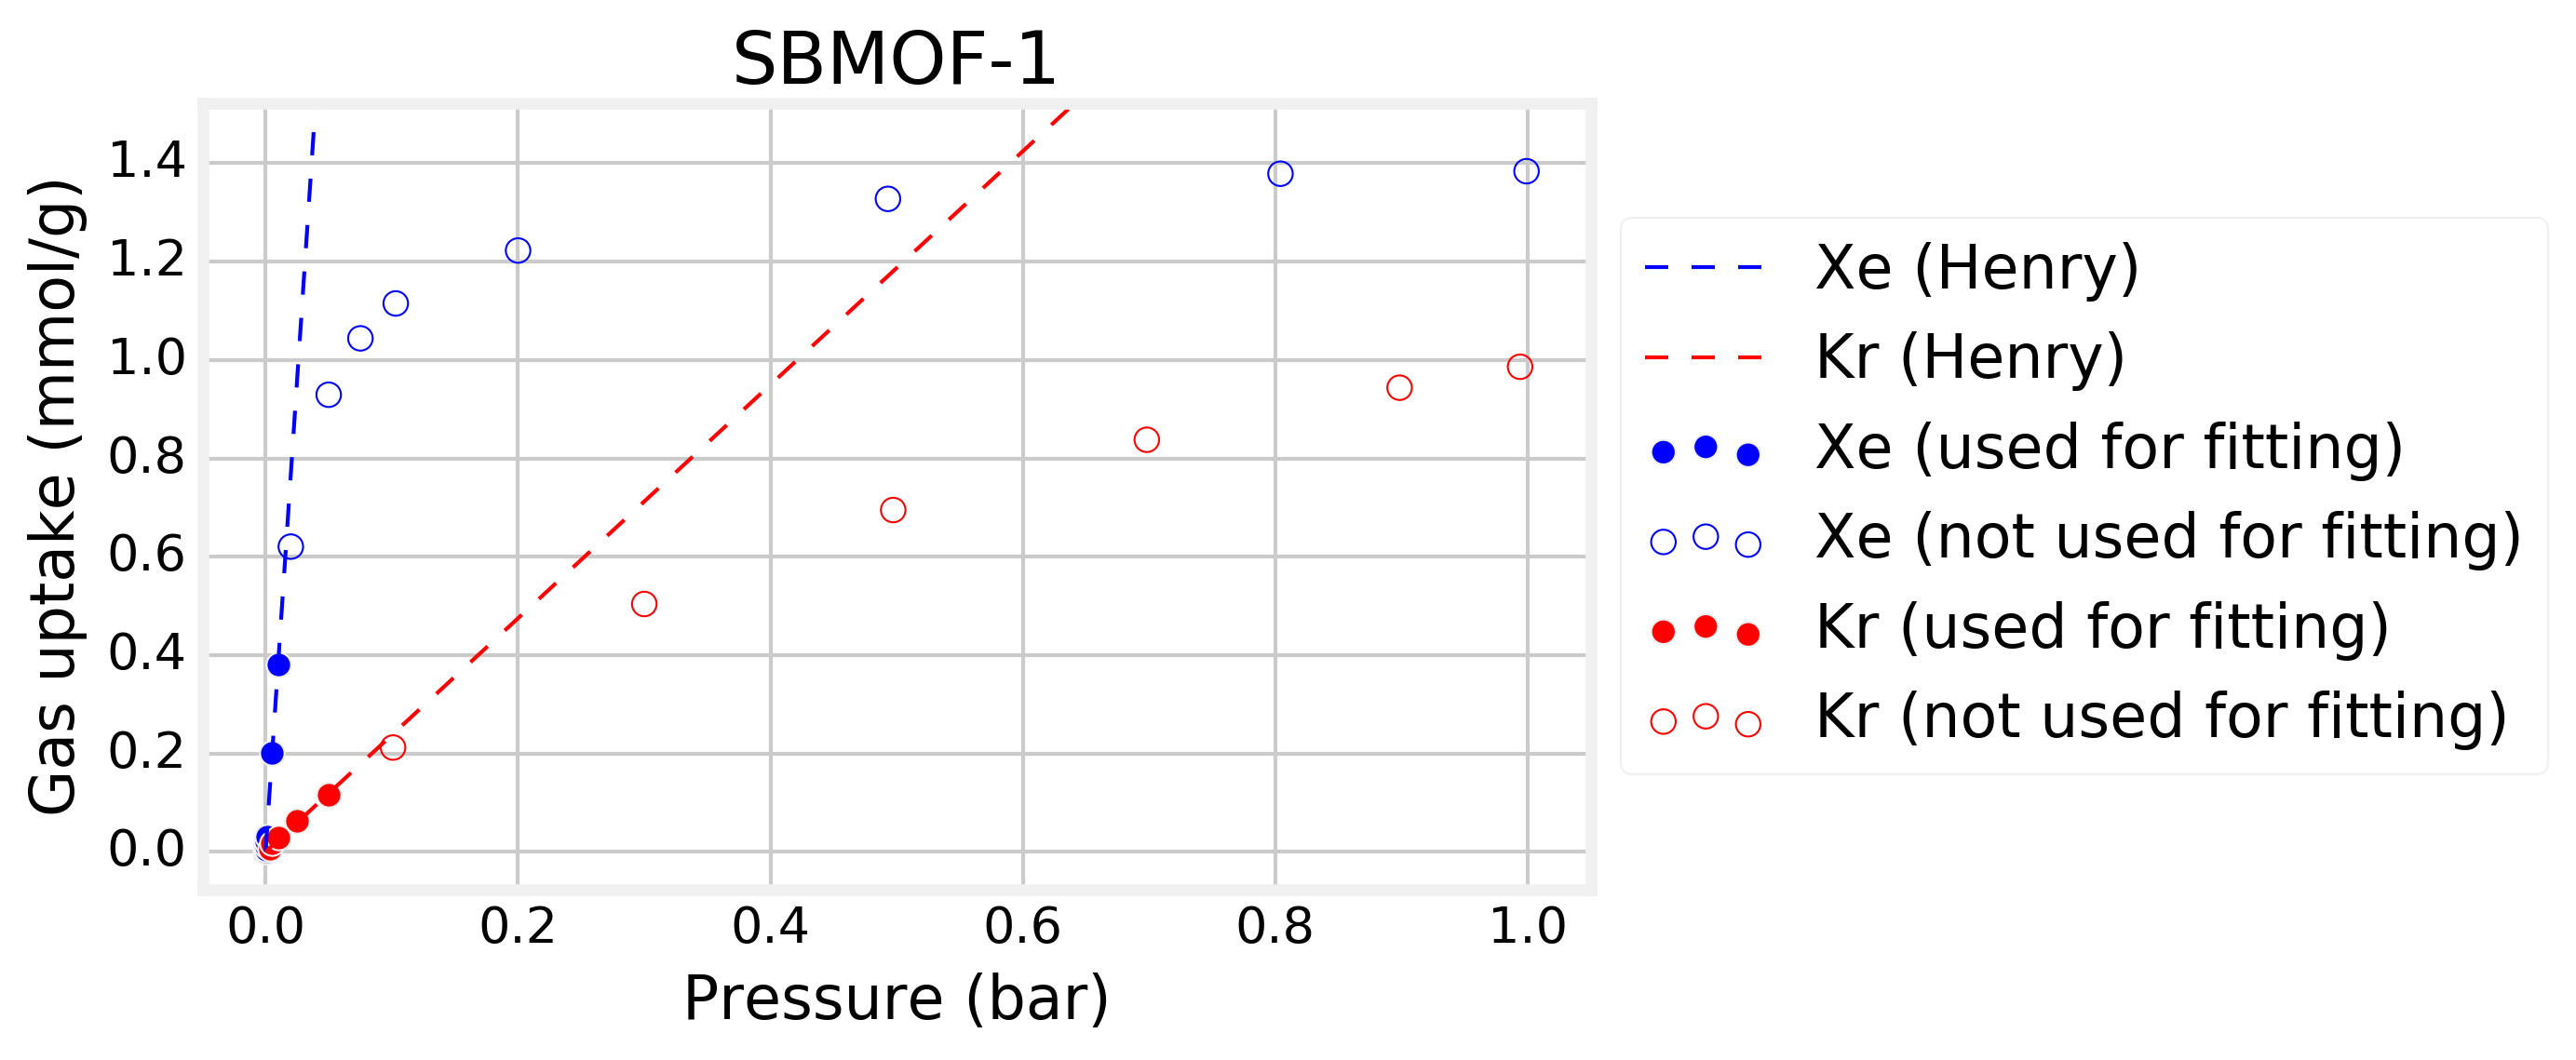
\includegraphics[width=.6\columnwidth]{../fits/SBMOF-1_fit.png} \label{fig:SBMOF-1_xtal} }
  
       \subfigure[]{\includegraphics[width=.45\columnwidth]{../fits/Xe_low_pressure_fit_SBMOF-1.png} \label{fig:SBMOF-1_Xe_KH} }
       \subfigure[]{\includegraphics[width=.45\columnwidth]{../fits/Kr_low_pressure_fit_SBMOF-1.png} \label{fig:SBMOF-1_Kr_KH} }
       
       \caption{SBMOF-1. (a) Crystal structure \cite{SBMOF-1_structure}.
       (b) Circles show pure-component Xe (blue) and Kr (red) adsorption isotherm data at 298 K from Ref. \cite{SBMOF-1_XeKr}. 
       Closed symbols are data used to identify the Henry coefficient. The dashed line shows Henry's law with the identified Henry coefficient.
       (c, d) Same as (b) but zoomed into the Henry regime. Identified Henry coefficient is shown in the box.}
    \end{figure}
    
    \clearpage
    
    
    \section{CC3}
    
    \begin{figure}[h!]
       \centering
       \subfigure[]{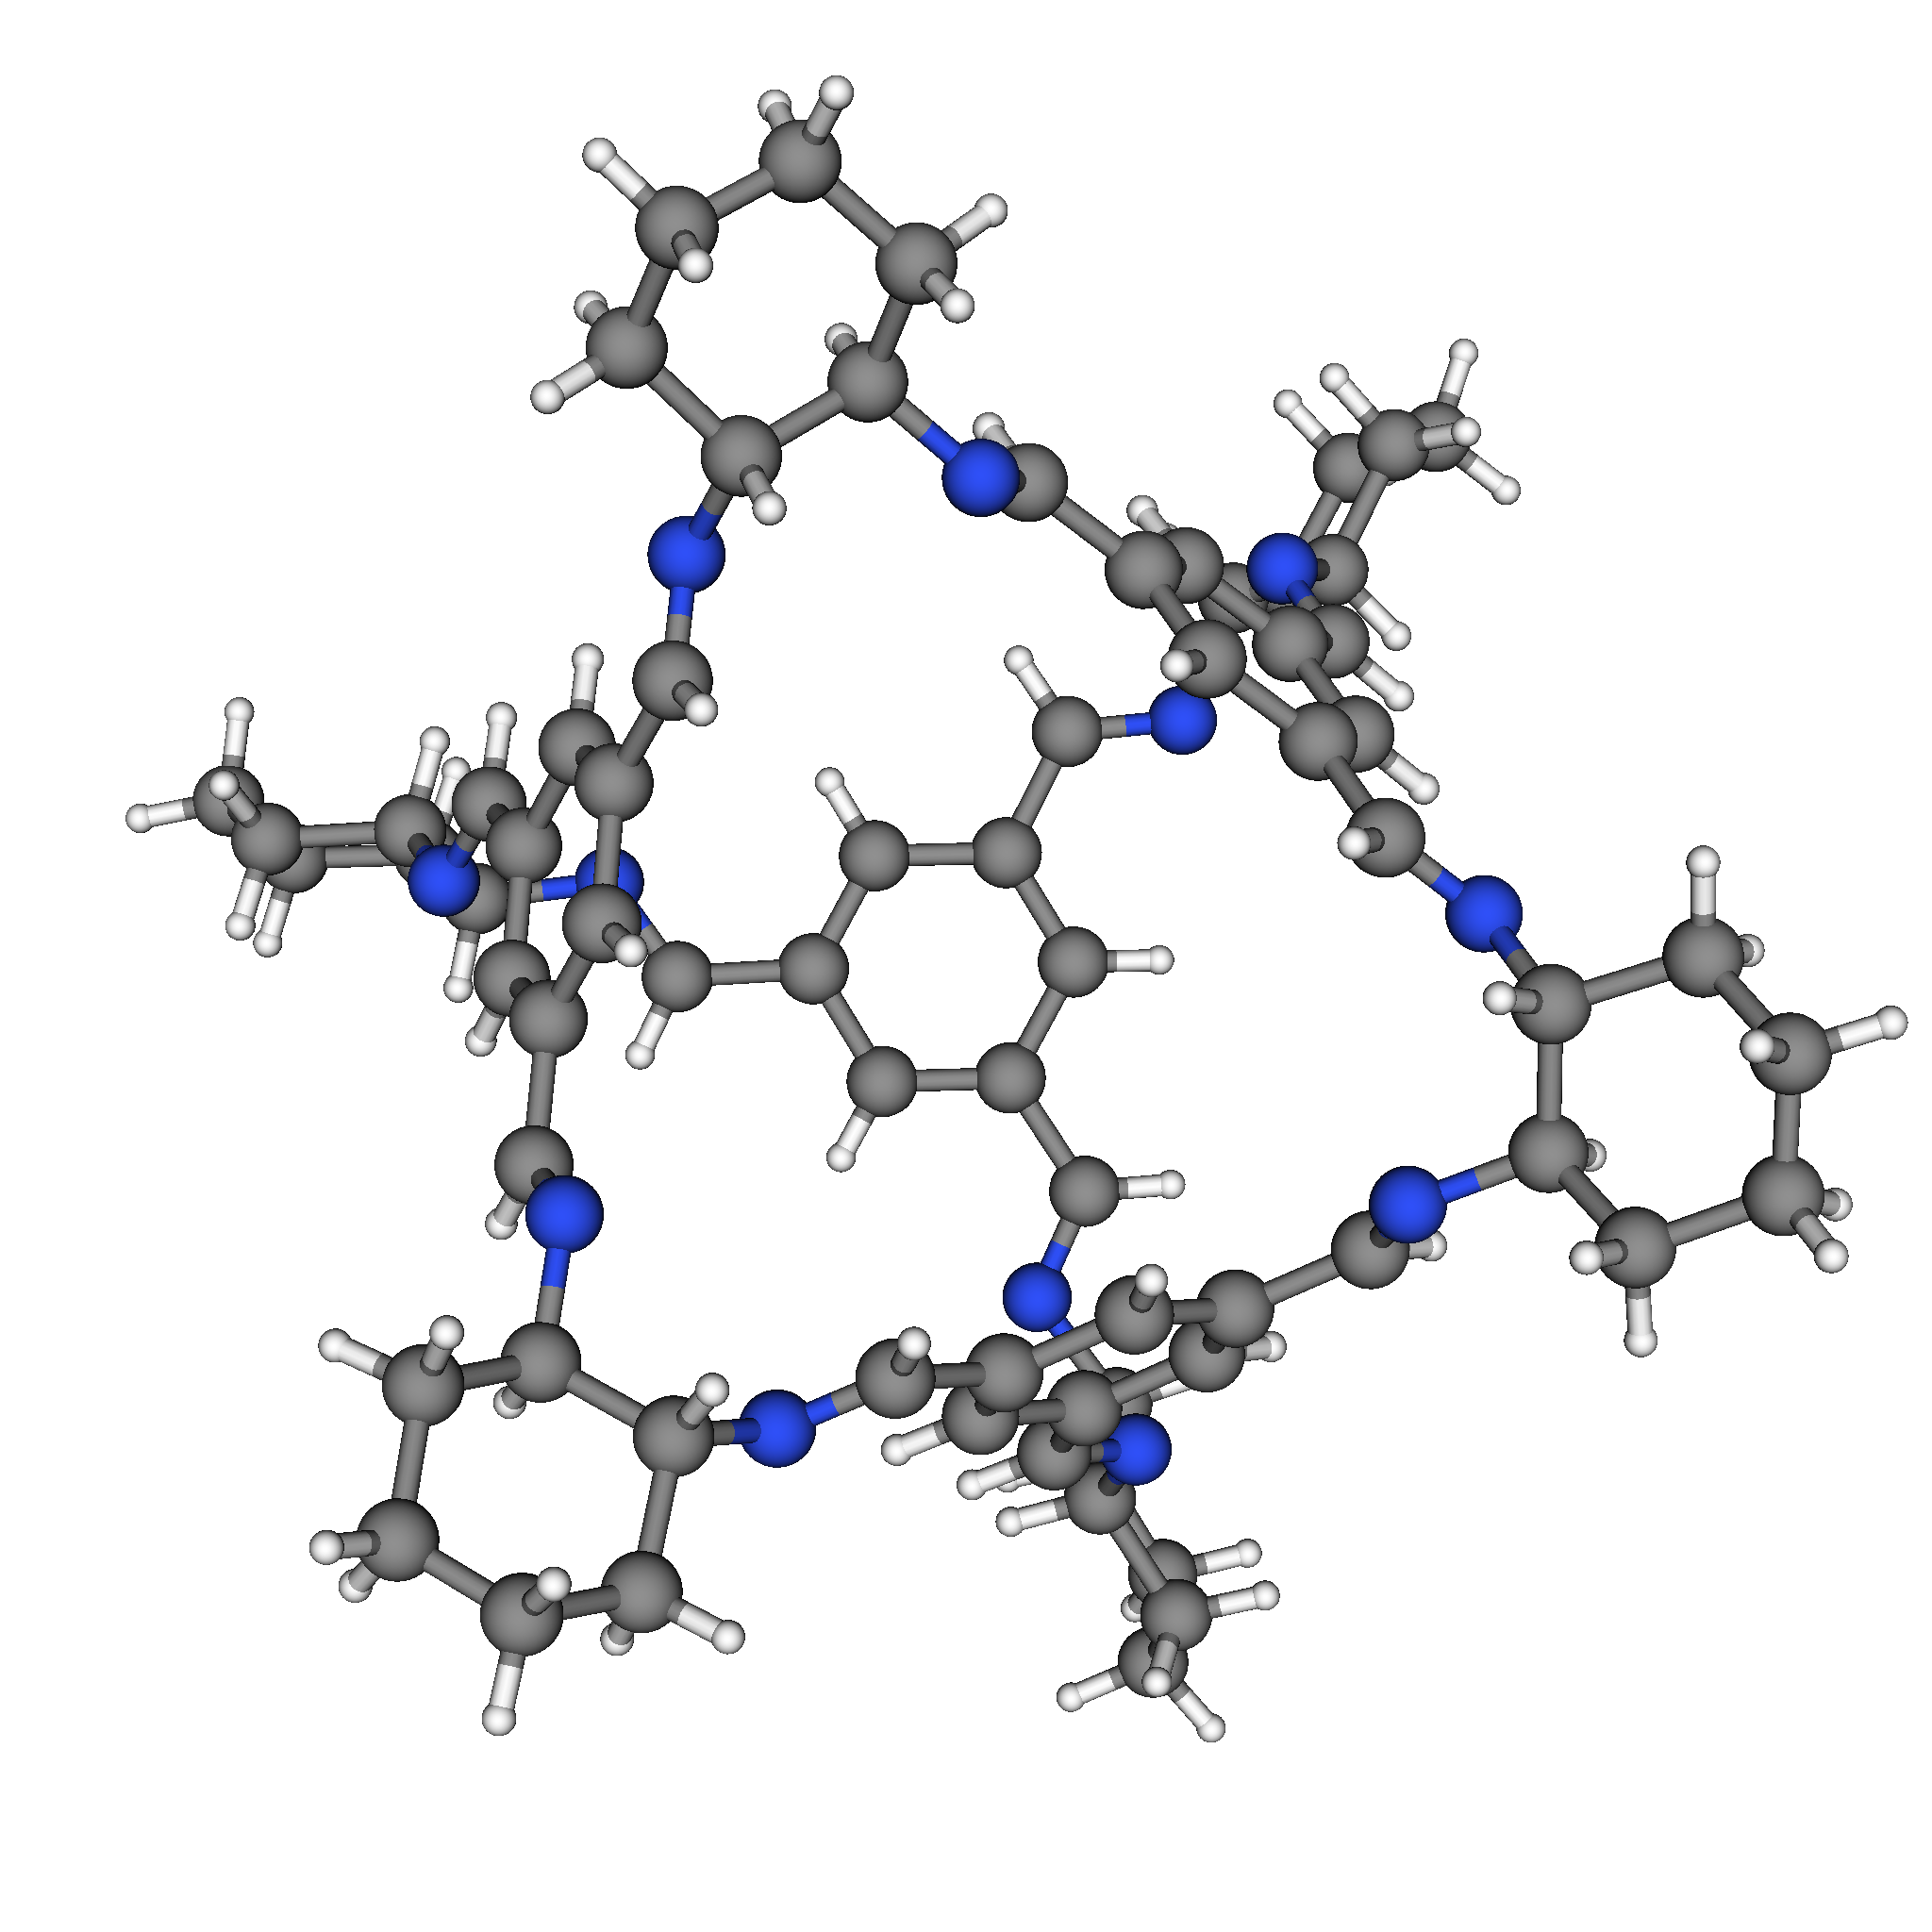
\includegraphics[width=.3\columnwidth]{../xtal_structures/viz/CC3.png} \label{fig:CC3_xtal} }
       \subfigure[]{\includegraphics[width=.6\columnwidth]{../fits/CC3_fit.png} \label{fig:CC3_xtal} }
  
       \subfigure[]{\includegraphics[width=.45\columnwidth]{../fits/Xe_low_pressure_fit_CC3.png} \label{fig:CC3_Xe_KH} }
       \subfigure[]{\includegraphics[width=.45\columnwidth]{../fits/Kr_low_pressure_fit_CC3.png} \label{fig:CC3_Kr_KH} }
       
       \caption{CC3. (a) Crystal structure \cite{CC3_structure}.
       (b) Circles show pure-component Xe (blue) and Kr (red) adsorption isotherm data at 298 K from Ref. \cite{CC3_XeKr}. 
       Closed symbols are data used to identify the Henry coefficient. The dashed line shows Henry's law with the identified Henry coefficient.
       (c, d) Same as (b) but zoomed into the Henry regime. Identified Henry coefficient is shown in the box.}
    \end{figure}
    
    \clearpage
    
    
    \section{IRMOF-1}
    
    \begin{figure}[h!]
       \centering
       \subfigure[]{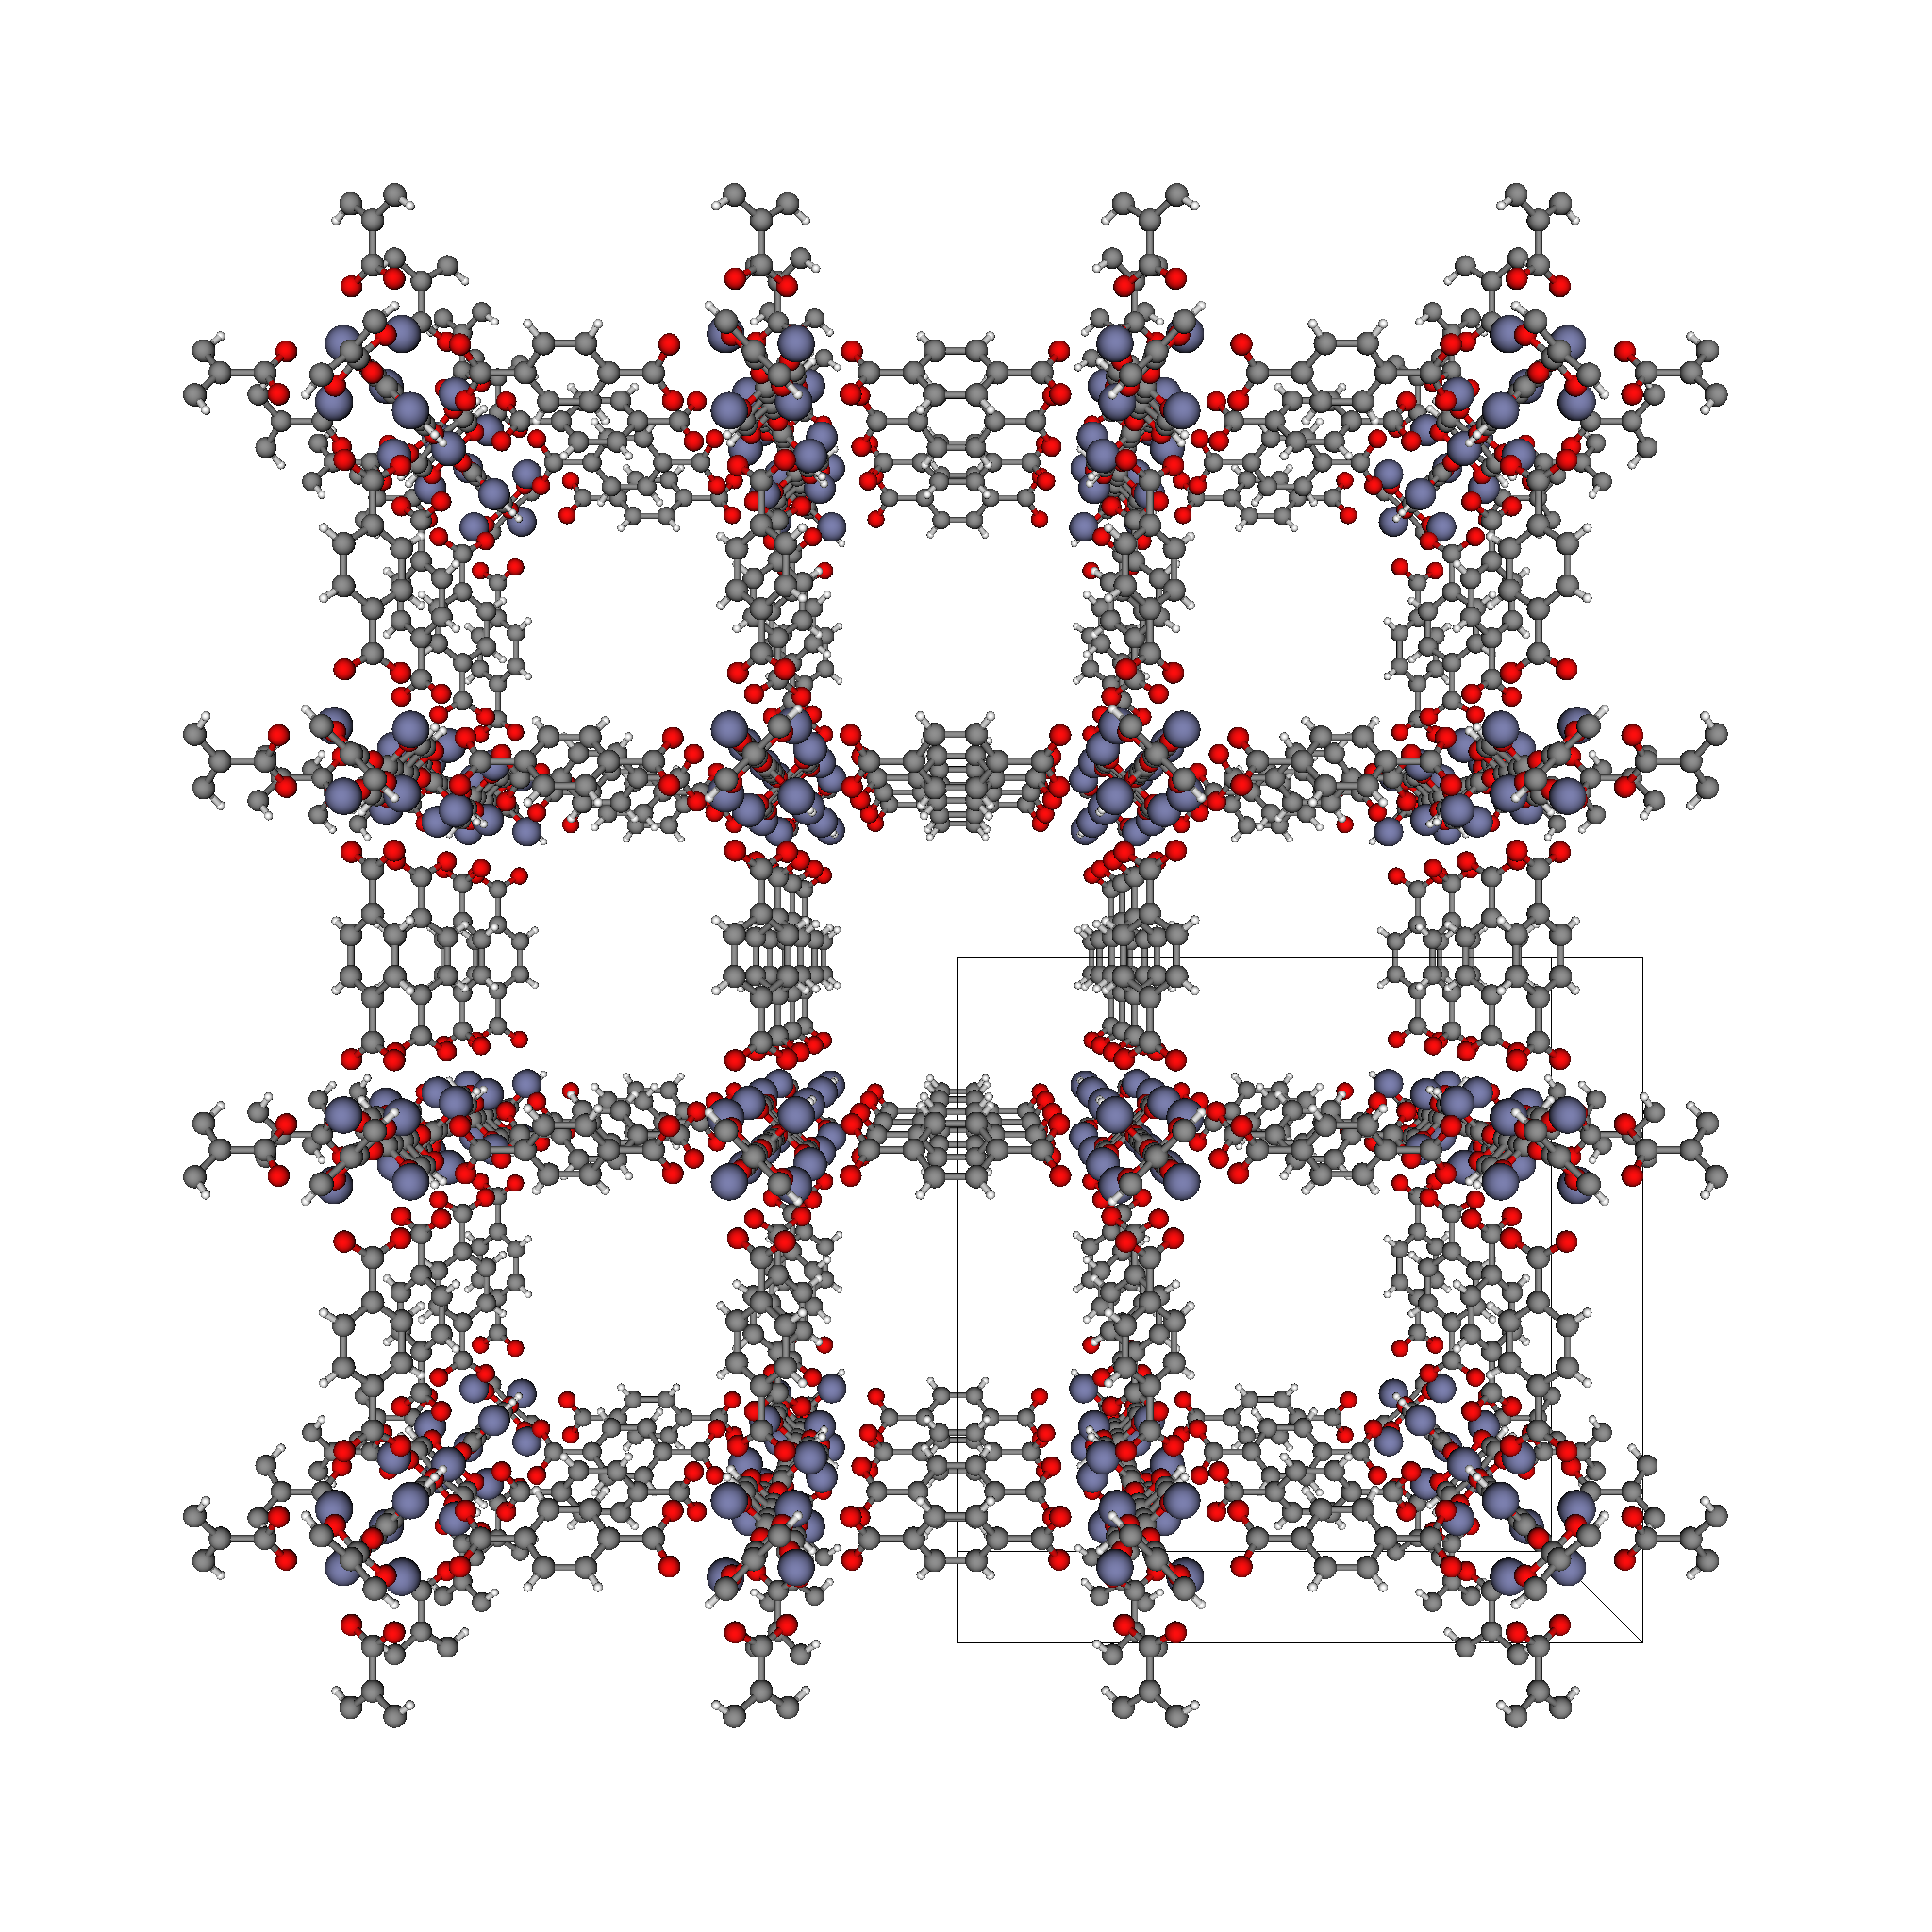
\includegraphics[width=.3\columnwidth]{../xtal_structures/viz/IRMOF-1.png} \label{fig:IRMOF-1_xtal} }
       \subfigure[]{\includegraphics[width=.6\columnwidth]{../fits/IRMOF-1_fit.png} \label{fig:IRMOF-1_xtal} }
  
       \subfigure[]{\includegraphics[width=.45\columnwidth]{../fits/Xe_low_pressure_fit_IRMOF-1.png} \label{fig:IRMOF-1_Xe_KH} }
       \subfigure[]{\includegraphics[width=.45\columnwidth]{../fits/Kr_low_pressure_fit_IRMOF-1.png} \label{fig:IRMOF-1_Kr_KH} }
       
       \caption{IRMOF-1. (a) Crystal structure \cite{IRMOF-1_structure}.
       (b) Circles show pure-component Xe (blue) and Kr (red) adsorption isotherm data at 292 K from Ref. \cite{IRMOF-1_XeKr}. 
       Closed symbols are data used to identify the Henry coefficient. The dashed line shows Henry's law with the identified Henry coefficient.
       (c, d) Same as (b) but zoomed into the Henry regime. Identified Henry coefficient is shown in the box.}
    \end{figure}
    
    \clearpage
    
    
    \section{Ni-MOF-74}
    
    \begin{figure}[h!]
       \centering
       \subfigure[]{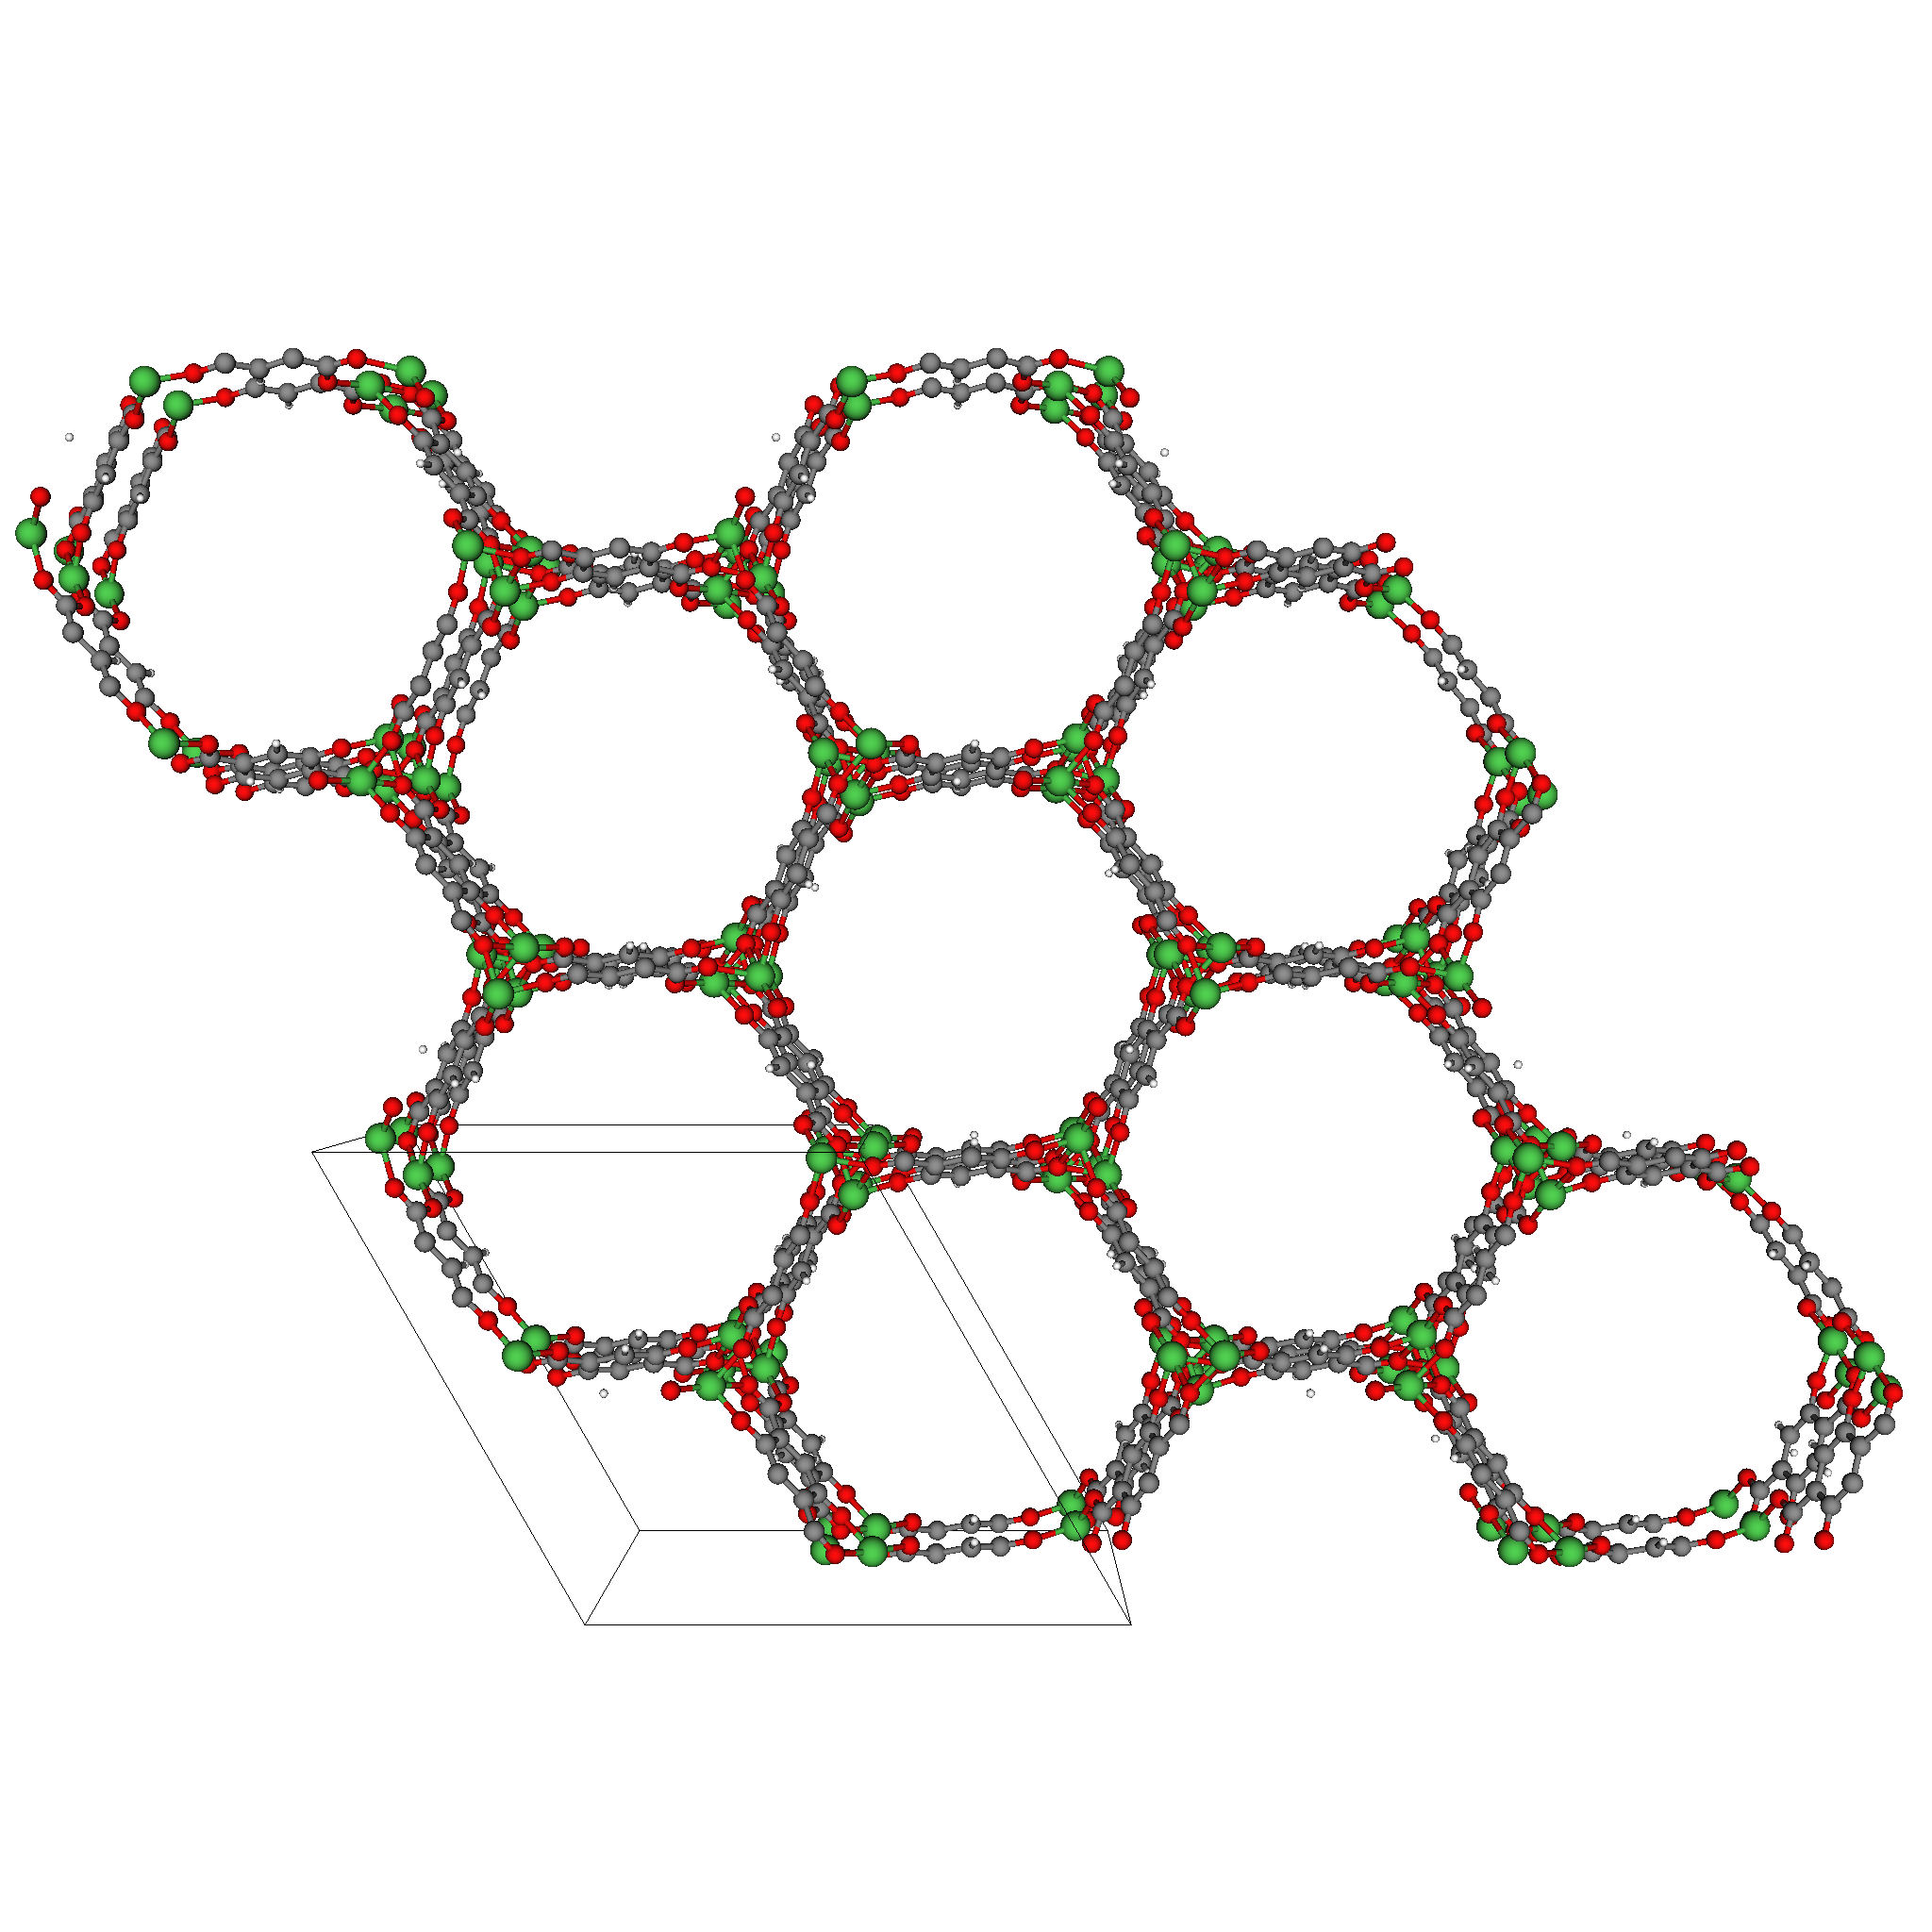
\includegraphics[width=.3\columnwidth]{../xtal_structures/viz/Ni-MOF-74.png} \label{fig:Ni-MOF-74_xtal} }
       \subfigure[]{\includegraphics[width=.6\columnwidth]{../fits/Ni-MOF-74_fit.png} \label{fig:Ni-MOF-74_xtal} }
  
       \subfigure[]{\includegraphics[width=.45\columnwidth]{../fits/Xe_low_pressure_fit_Ni-MOF-74.png} \label{fig:Ni-MOF-74_Xe_KH} }
       \subfigure[]{\includegraphics[width=.45\columnwidth]{../fits/Kr_low_pressure_fit_Ni-MOF-74.png} \label{fig:Ni-MOF-74_Kr_KH} }
       
       \caption{Ni-MOF-74. (a) Crystal structure \cite{Ni-MOF-74_structure}.
       (b) Circles show pure-component Xe (blue) and Kr (red) adsorption isotherm data at 298 K from Ref. \cite{Ni-MOF-74_XeKr}. 
       Closed symbols are data used to identify the Henry coefficient. The dashed line shows Henry's law with the identified Henry coefficient.
       (c, d) Same as (b) but zoomed into the Henry regime. Identified Henry coefficient is shown in the box.}
    \end{figure}
    
    \clearpage
    
    
    \section{HKUST-1}
    
    \begin{figure}[h!]
       \centering
       \subfigure[]{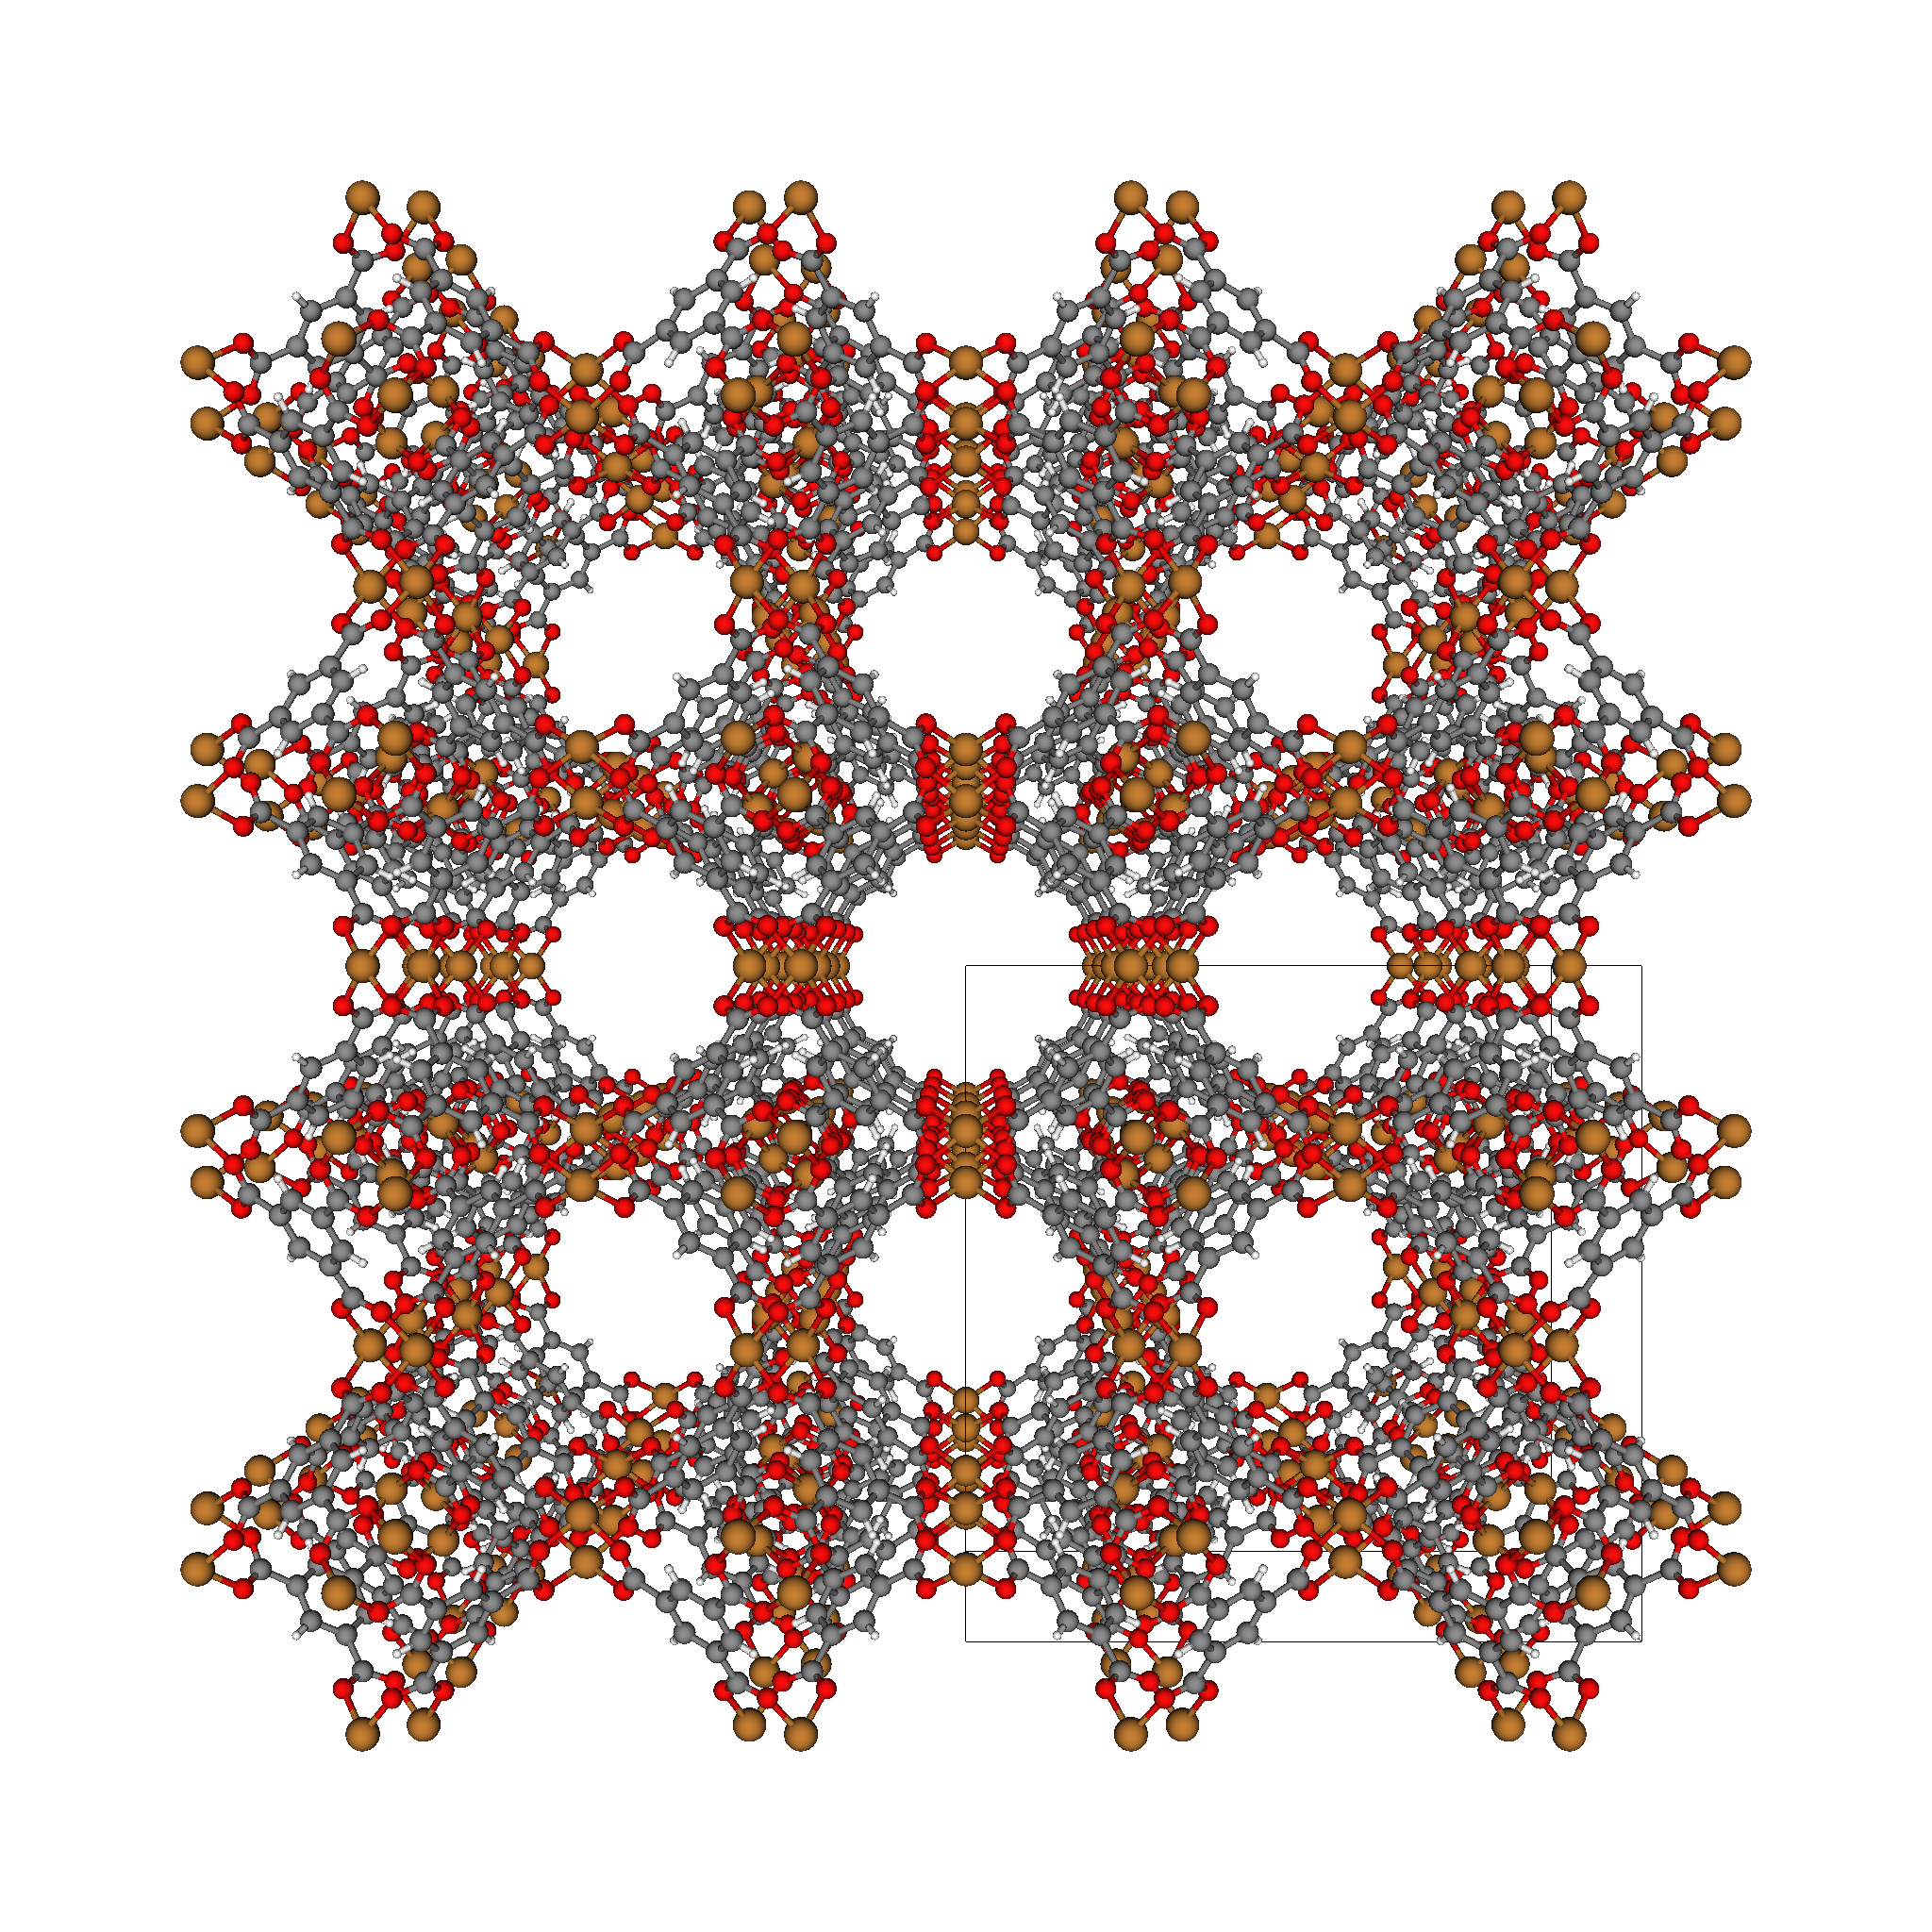
\includegraphics[width=.3\columnwidth]{../xtal_structures/viz/HKUST-1.png} \label{fig:HKUST-1_xtal} }
       \subfigure[]{\includegraphics[width=.6\columnwidth]{../fits/HKUST-1_fit.png} \label{fig:HKUST-1_xtal} }
  
       \subfigure[]{\includegraphics[width=.45\columnwidth]{../fits/Xe_low_pressure_fit_HKUST-1.png} \label{fig:HKUST-1_Xe_KH} }
       \subfigure[]{\includegraphics[width=.45\columnwidth]{../fits/Kr_low_pressure_fit_HKUST-1.png} \label{fig:HKUST-1_Kr_KH} }
       
       \caption{HKUST-1. (a) Crystal structure \cite{HKUST-1_structure}.
       (b) Circles show pure-component Xe (blue) and Kr (red) adsorption isotherm data at 298 K from Ref. \cite{HKUST-1_XeKr}. 
       Closed symbols are data used to identify the Henry coefficient. The dashed line shows Henry's law with the identified Henry coefficient.
       (c, d) Same as (b) but zoomed into the Henry regime. Identified Henry coefficient is shown in the box.}
    \end{figure}
    
    \clearpage
    
    
    \section{SBMOF-2}
    
    \begin{figure}[h!]
       \centering
       \subfigure[]{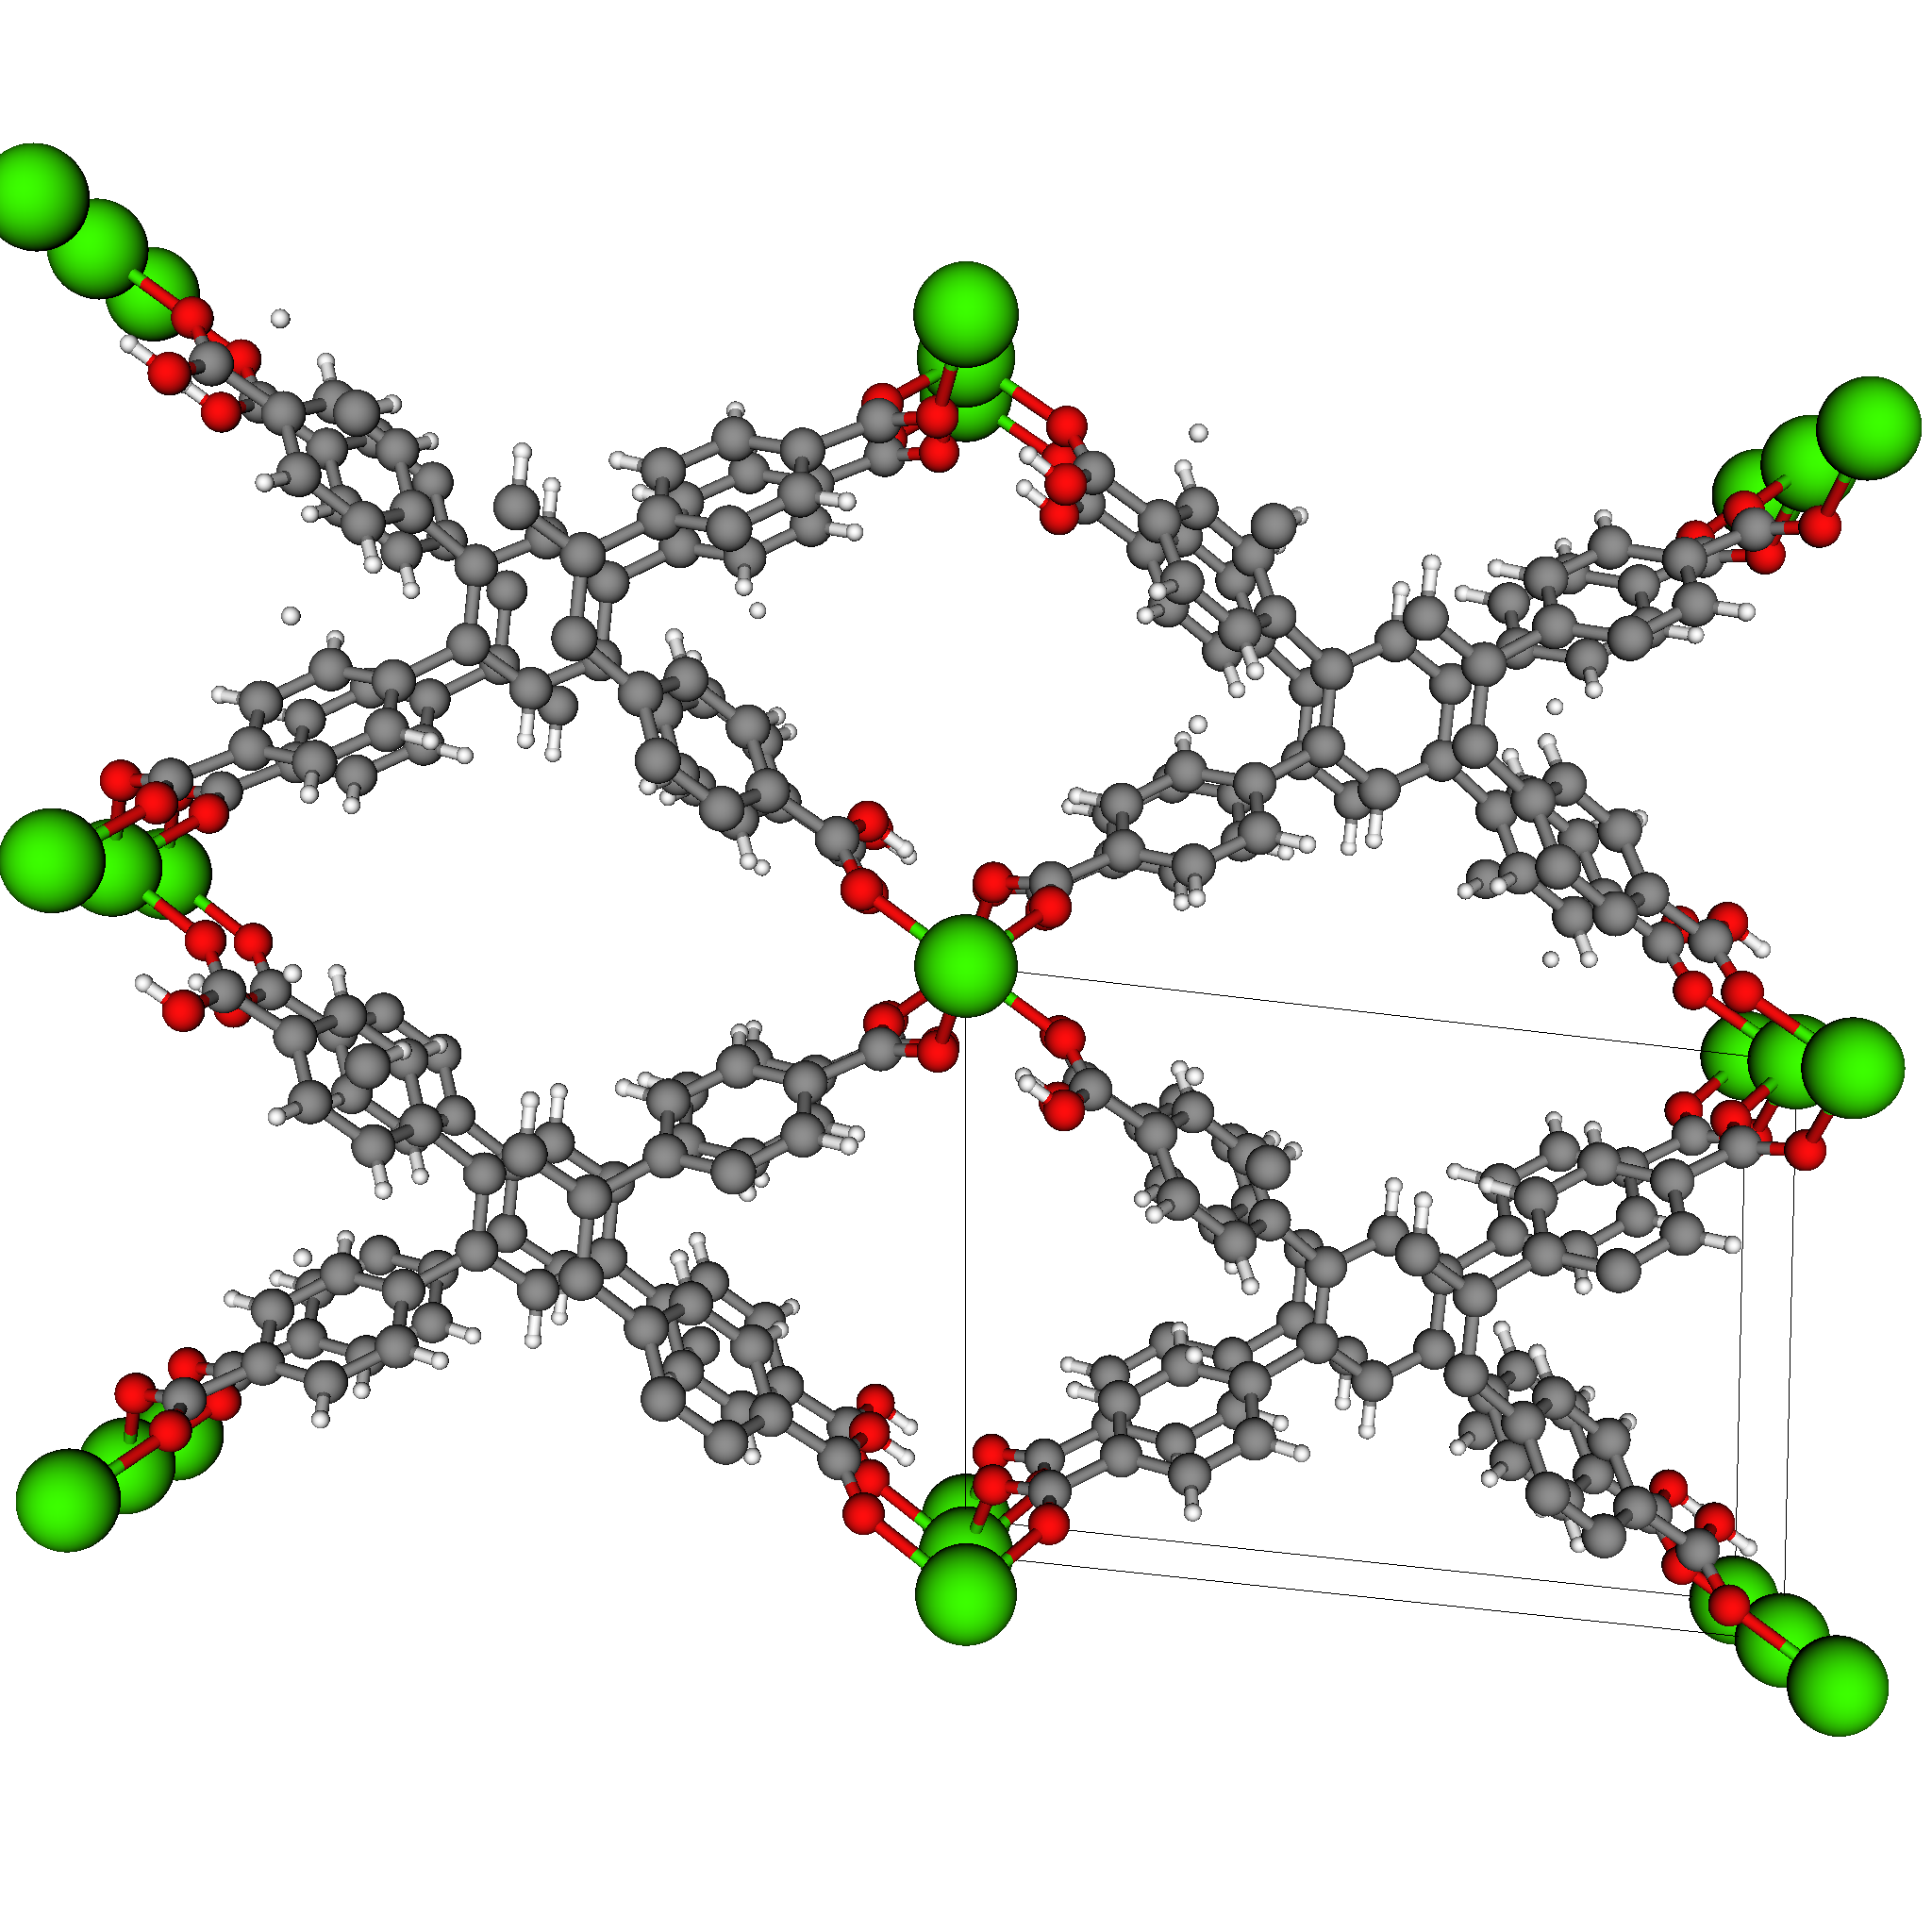
\includegraphics[width=.3\columnwidth]{../xtal_structures/viz/SBMOF-2.png} \label{fig:SBMOF-2_xtal} }
       \subfigure[]{\includegraphics[width=.6\columnwidth]{../fits/SBMOF-2_fit.png} \label{fig:SBMOF-2_xtal} }
  
       \subfigure[]{\includegraphics[width=.45\columnwidth]{../fits/Xe_low_pressure_fit_SBMOF-2.png} \label{fig:SBMOF-2_Xe_KH} }
       \subfigure[]{\includegraphics[width=.45\columnwidth]{../fits/Kr_low_pressure_fit_SBMOF-2.png} \label{fig:SBMOF-2_Kr_KH} }
       
       \caption{SBMOF-2. (a) Crystal structure \cite{SBMOF-2_structure}.
       (b) Circles show pure-component Xe (blue) and Kr (red) adsorption isotherm data at 298 K from Ref. \cite{SBMOF-2_XeKr}. 
       Closed symbols are data used to identify the Henry coefficient. The dashed line shows Henry's law with the identified Henry coefficient.
       (c, d) Same as (b) but zoomed into the Henry regime. Identified Henry coefficient is shown in the box.}
    \end{figure}
    
    \clearpage
    
    
    \section{Co-formate}
    
    \begin{figure}[h!]
       \centering
       \subfigure[]{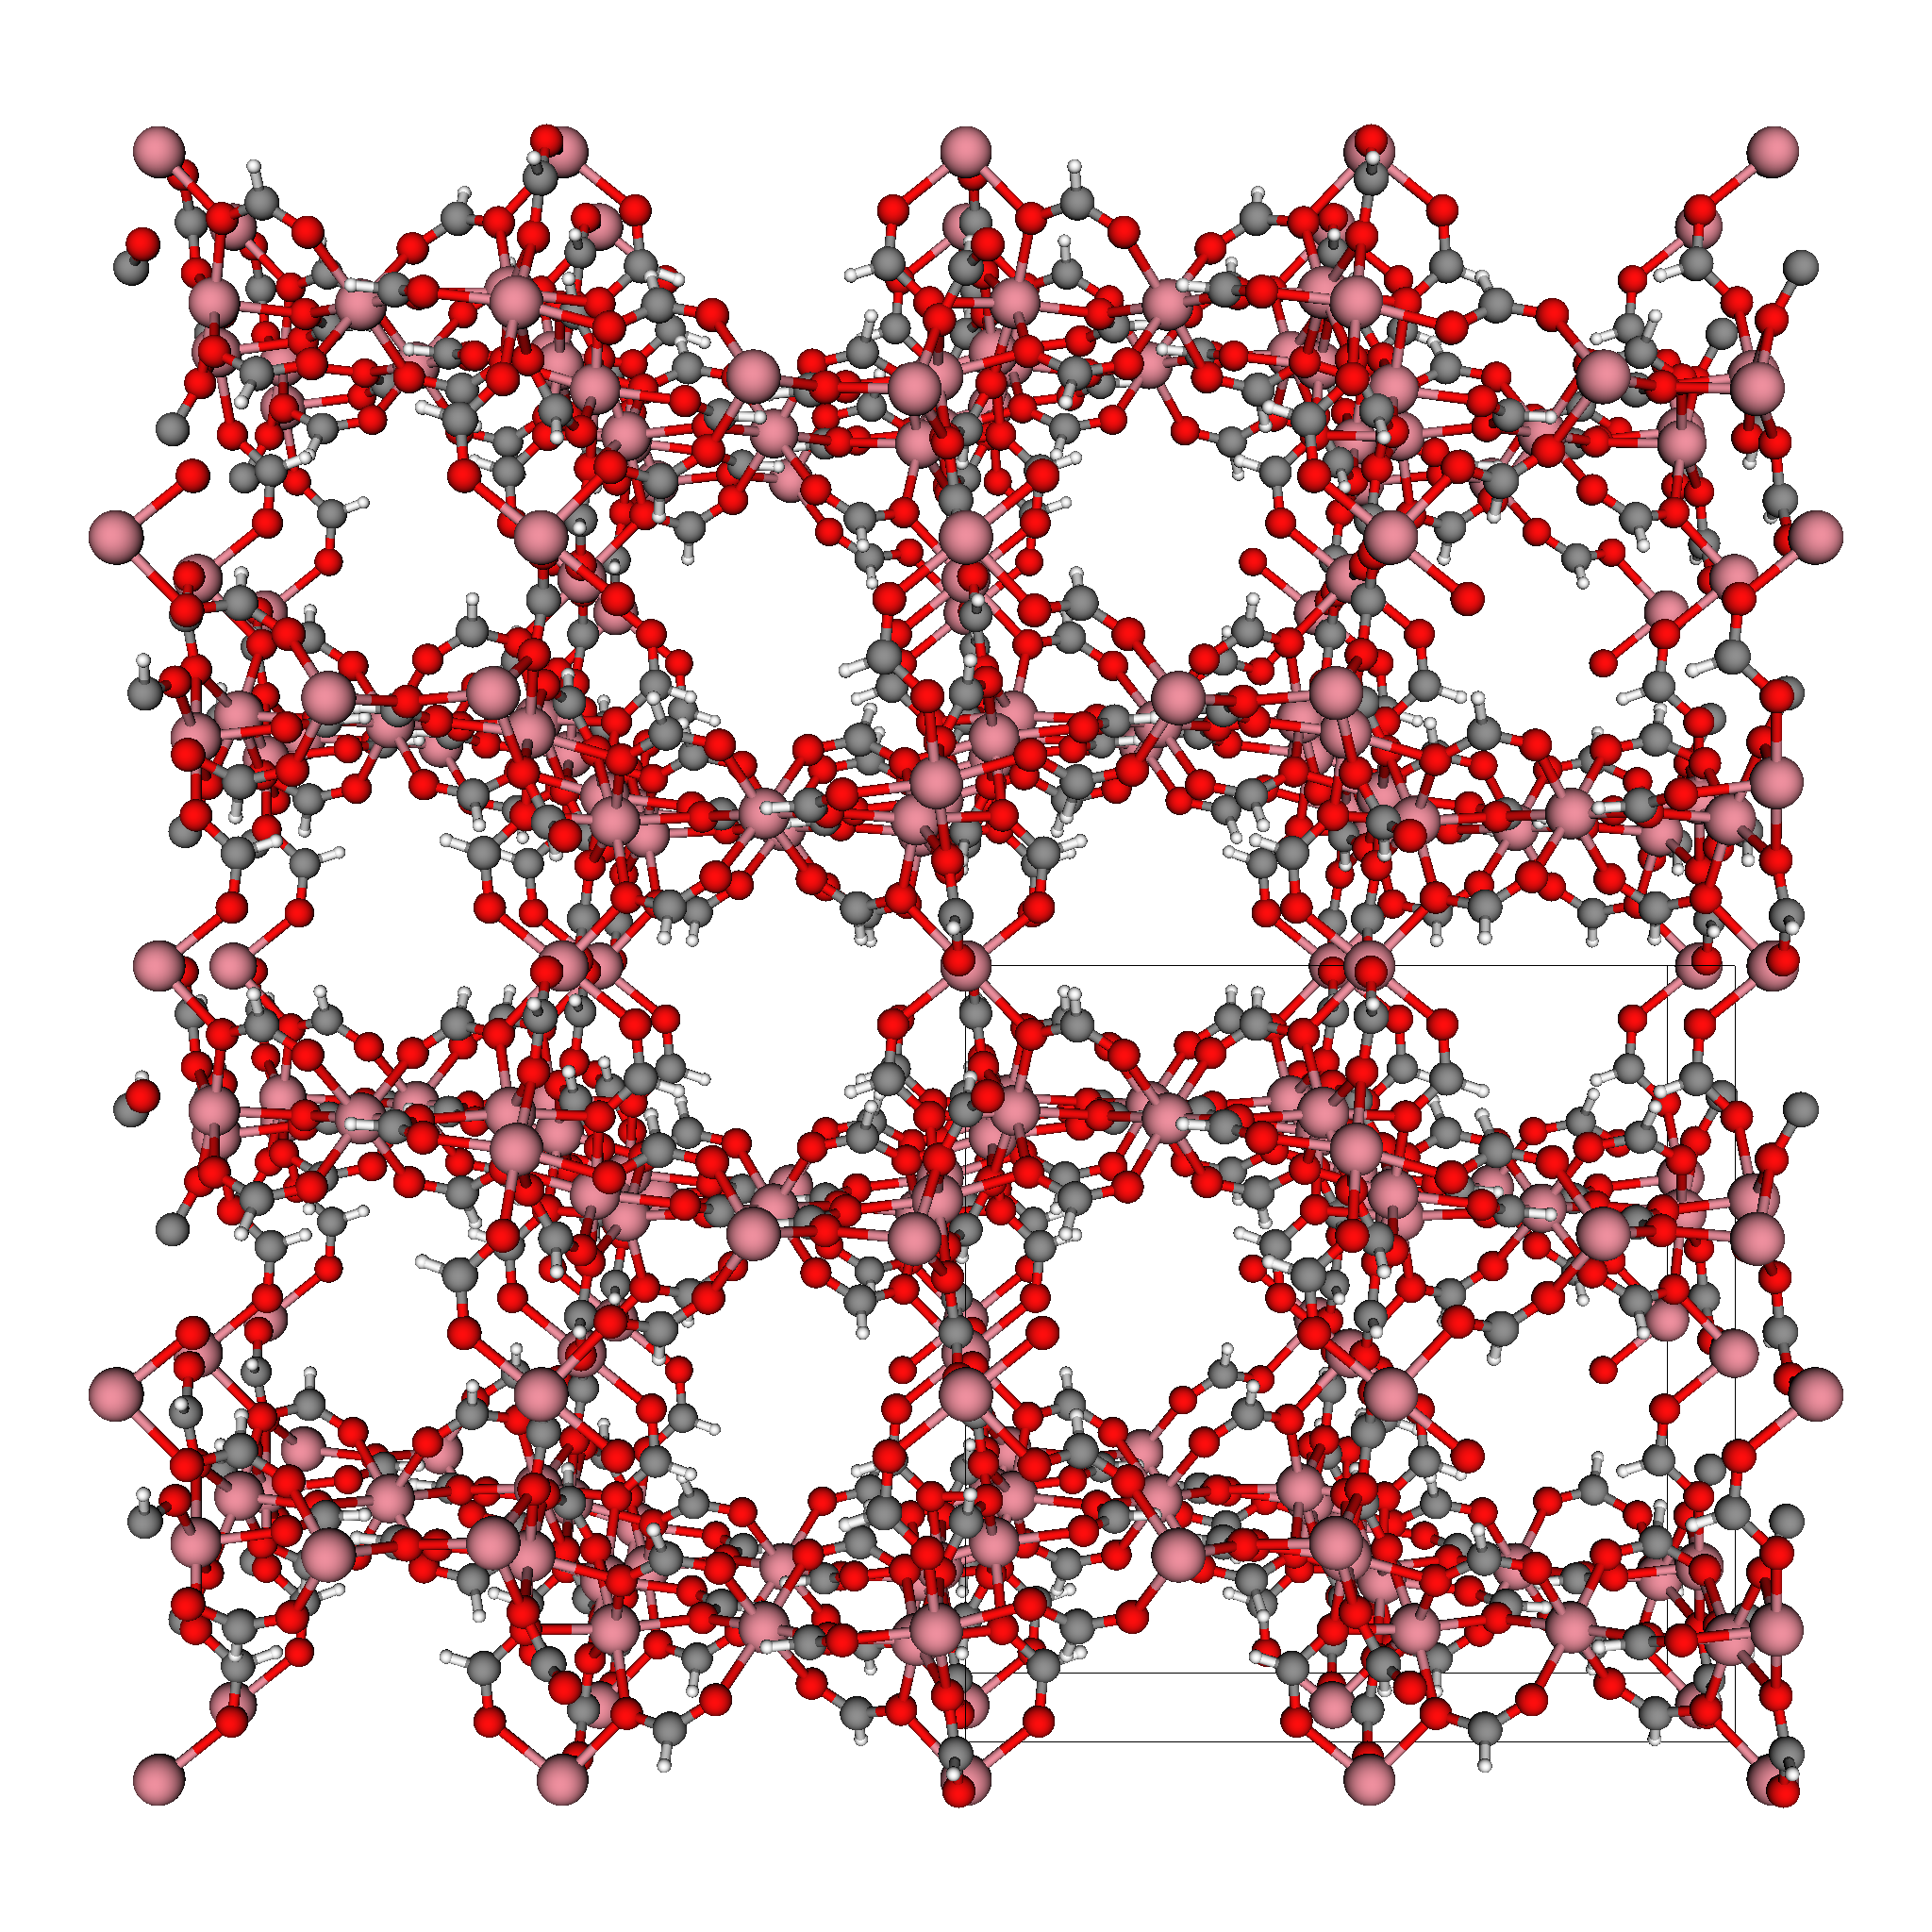
\includegraphics[width=.3\columnwidth]{../xtal_structures/viz/Co-formate.png} \label{fig:Co-formate_xtal} }
       \subfigure[]{\includegraphics[width=.6\columnwidth]{../fits/Co-formate_fit.png} \label{fig:Co-formate_xtal} }
  
       \subfigure[]{\includegraphics[width=.45\columnwidth]{../fits/Xe_low_pressure_fit_Co-formate.png} \label{fig:Co-formate_Xe_KH} }
       \subfigure[]{\includegraphics[width=.45\columnwidth]{../fits/Kr_low_pressure_fit_Co-formate.png} \label{fig:Co-formate_Kr_KH} }
       
       \caption{Co-formate. (a) Crystal structure \cite{Co-formate_structure}.
       (b) Circles show pure-component Xe (blue) and Kr (red) adsorption isotherm data at 298 K from Ref. \cite{Co-formate_XeKr}. 
       Closed symbols are data used to identify the Henry coefficient. The dashed line shows Henry's law with the identified Henry coefficient.
       (c, d) Same as (b) but zoomed into the Henry regime. Identified Henry coefficient is shown in the box.}
    \end{figure}
    
    \clearpage
    
    
    \section{ZincTetrazolate}
    
    \begin{figure}[h!]
       \centering
       \subfigure[]{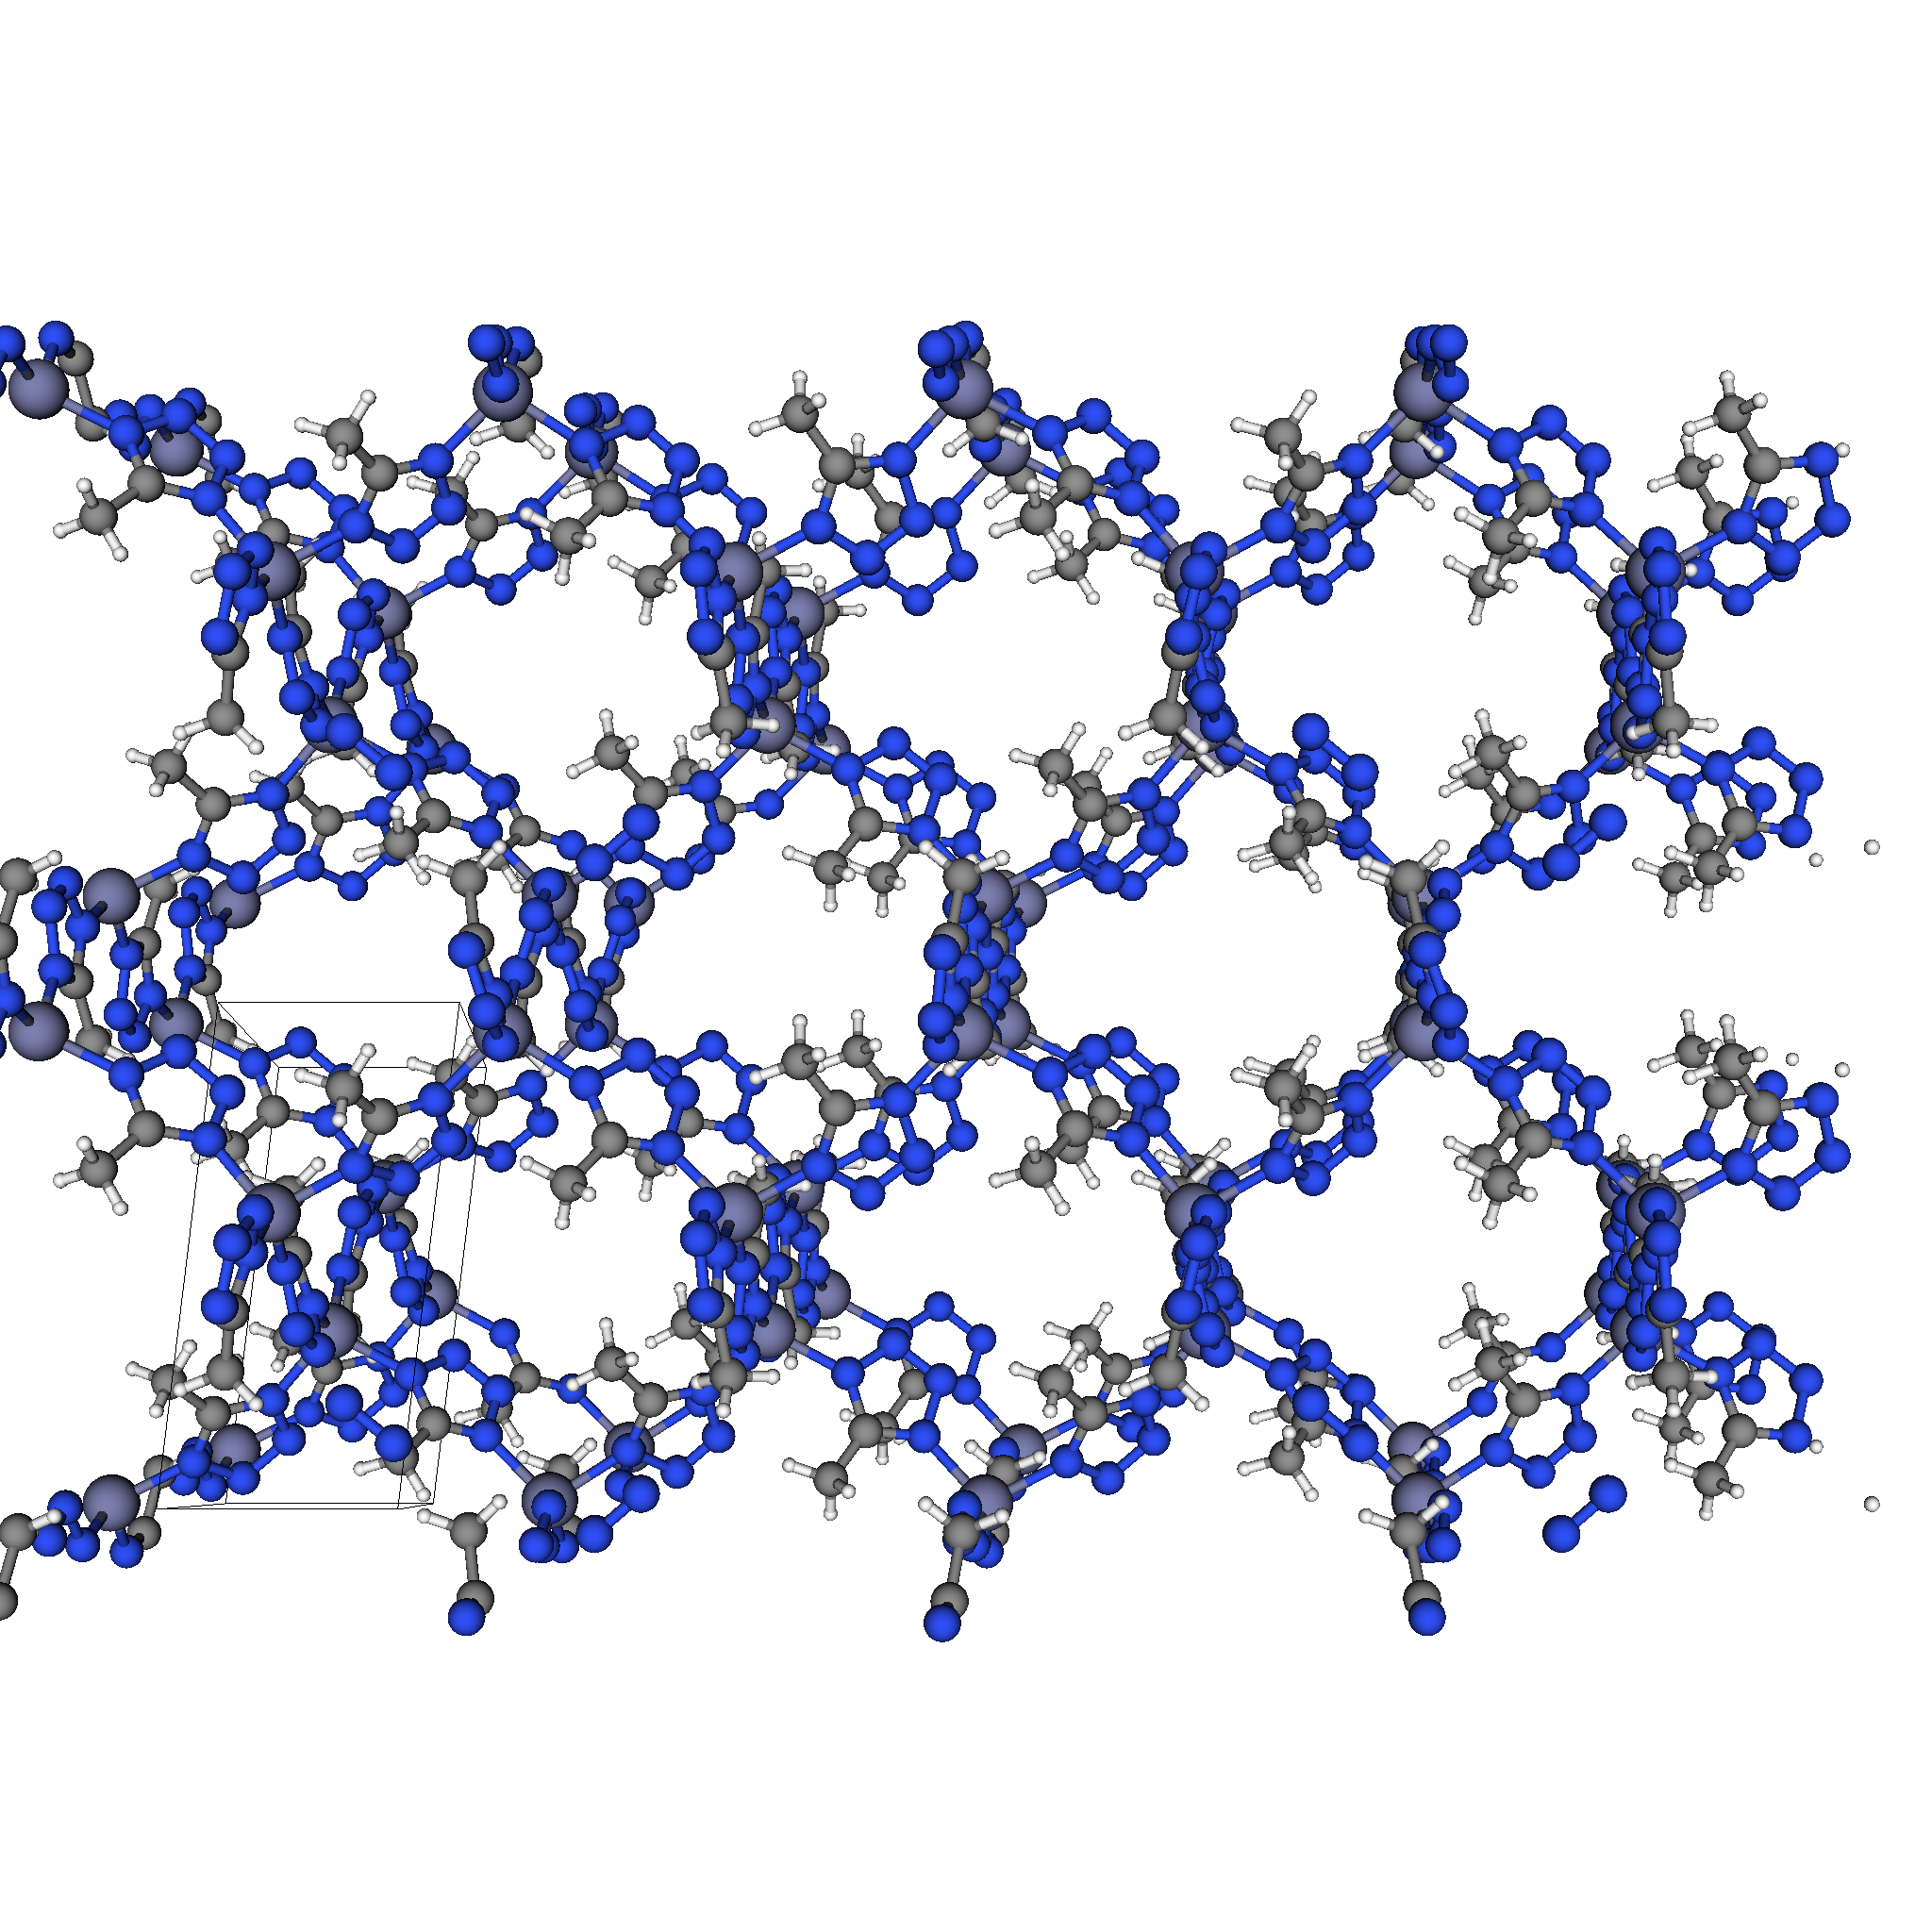
\includegraphics[width=.3\columnwidth]{../xtal_structures/viz/ZincTetrazolate.png} \label{fig:ZincTetrazolate_xtal} }
       \subfigure[]{\includegraphics[width=.6\columnwidth]{../fits/ZincTetrazolate_fit.png} \label{fig:ZincTetrazolate_xtal} }
  
       \subfigure[]{\includegraphics[width=.45\columnwidth]{../fits/Xe_low_pressure_fit_ZincTetrazolate.png} \label{fig:ZincTetrazolate_Xe_KH} }
       \subfigure[]{\includegraphics[width=.45\columnwidth]{../fits/Kr_low_pressure_fit_ZincTetrazolate.png} \label{fig:ZincTetrazolate_Kr_KH} }
       
       \caption{ZincTetrazolate. (a) Crystal structure \cite{ZincTetrazolate_structure}.
       (b) Circles show pure-component Xe (blue) and Kr (red) adsorption isotherm data at 298 K from Ref. \cite{ZincTetrazolate_XeKr}. 
       Closed symbols are data used to identify the Henry coefficient. The dashed line shows Henry's law with the identified Henry coefficient.
       (c, d) Same as (b) but zoomed into the Henry regime. Identified Henry coefficient is shown in the box.}
    \end{figure}
    
    \clearpage
    
    
    \section{FMOF-Cu}
    
    \begin{figure}[h!]
       \centering
       \subfigure[]{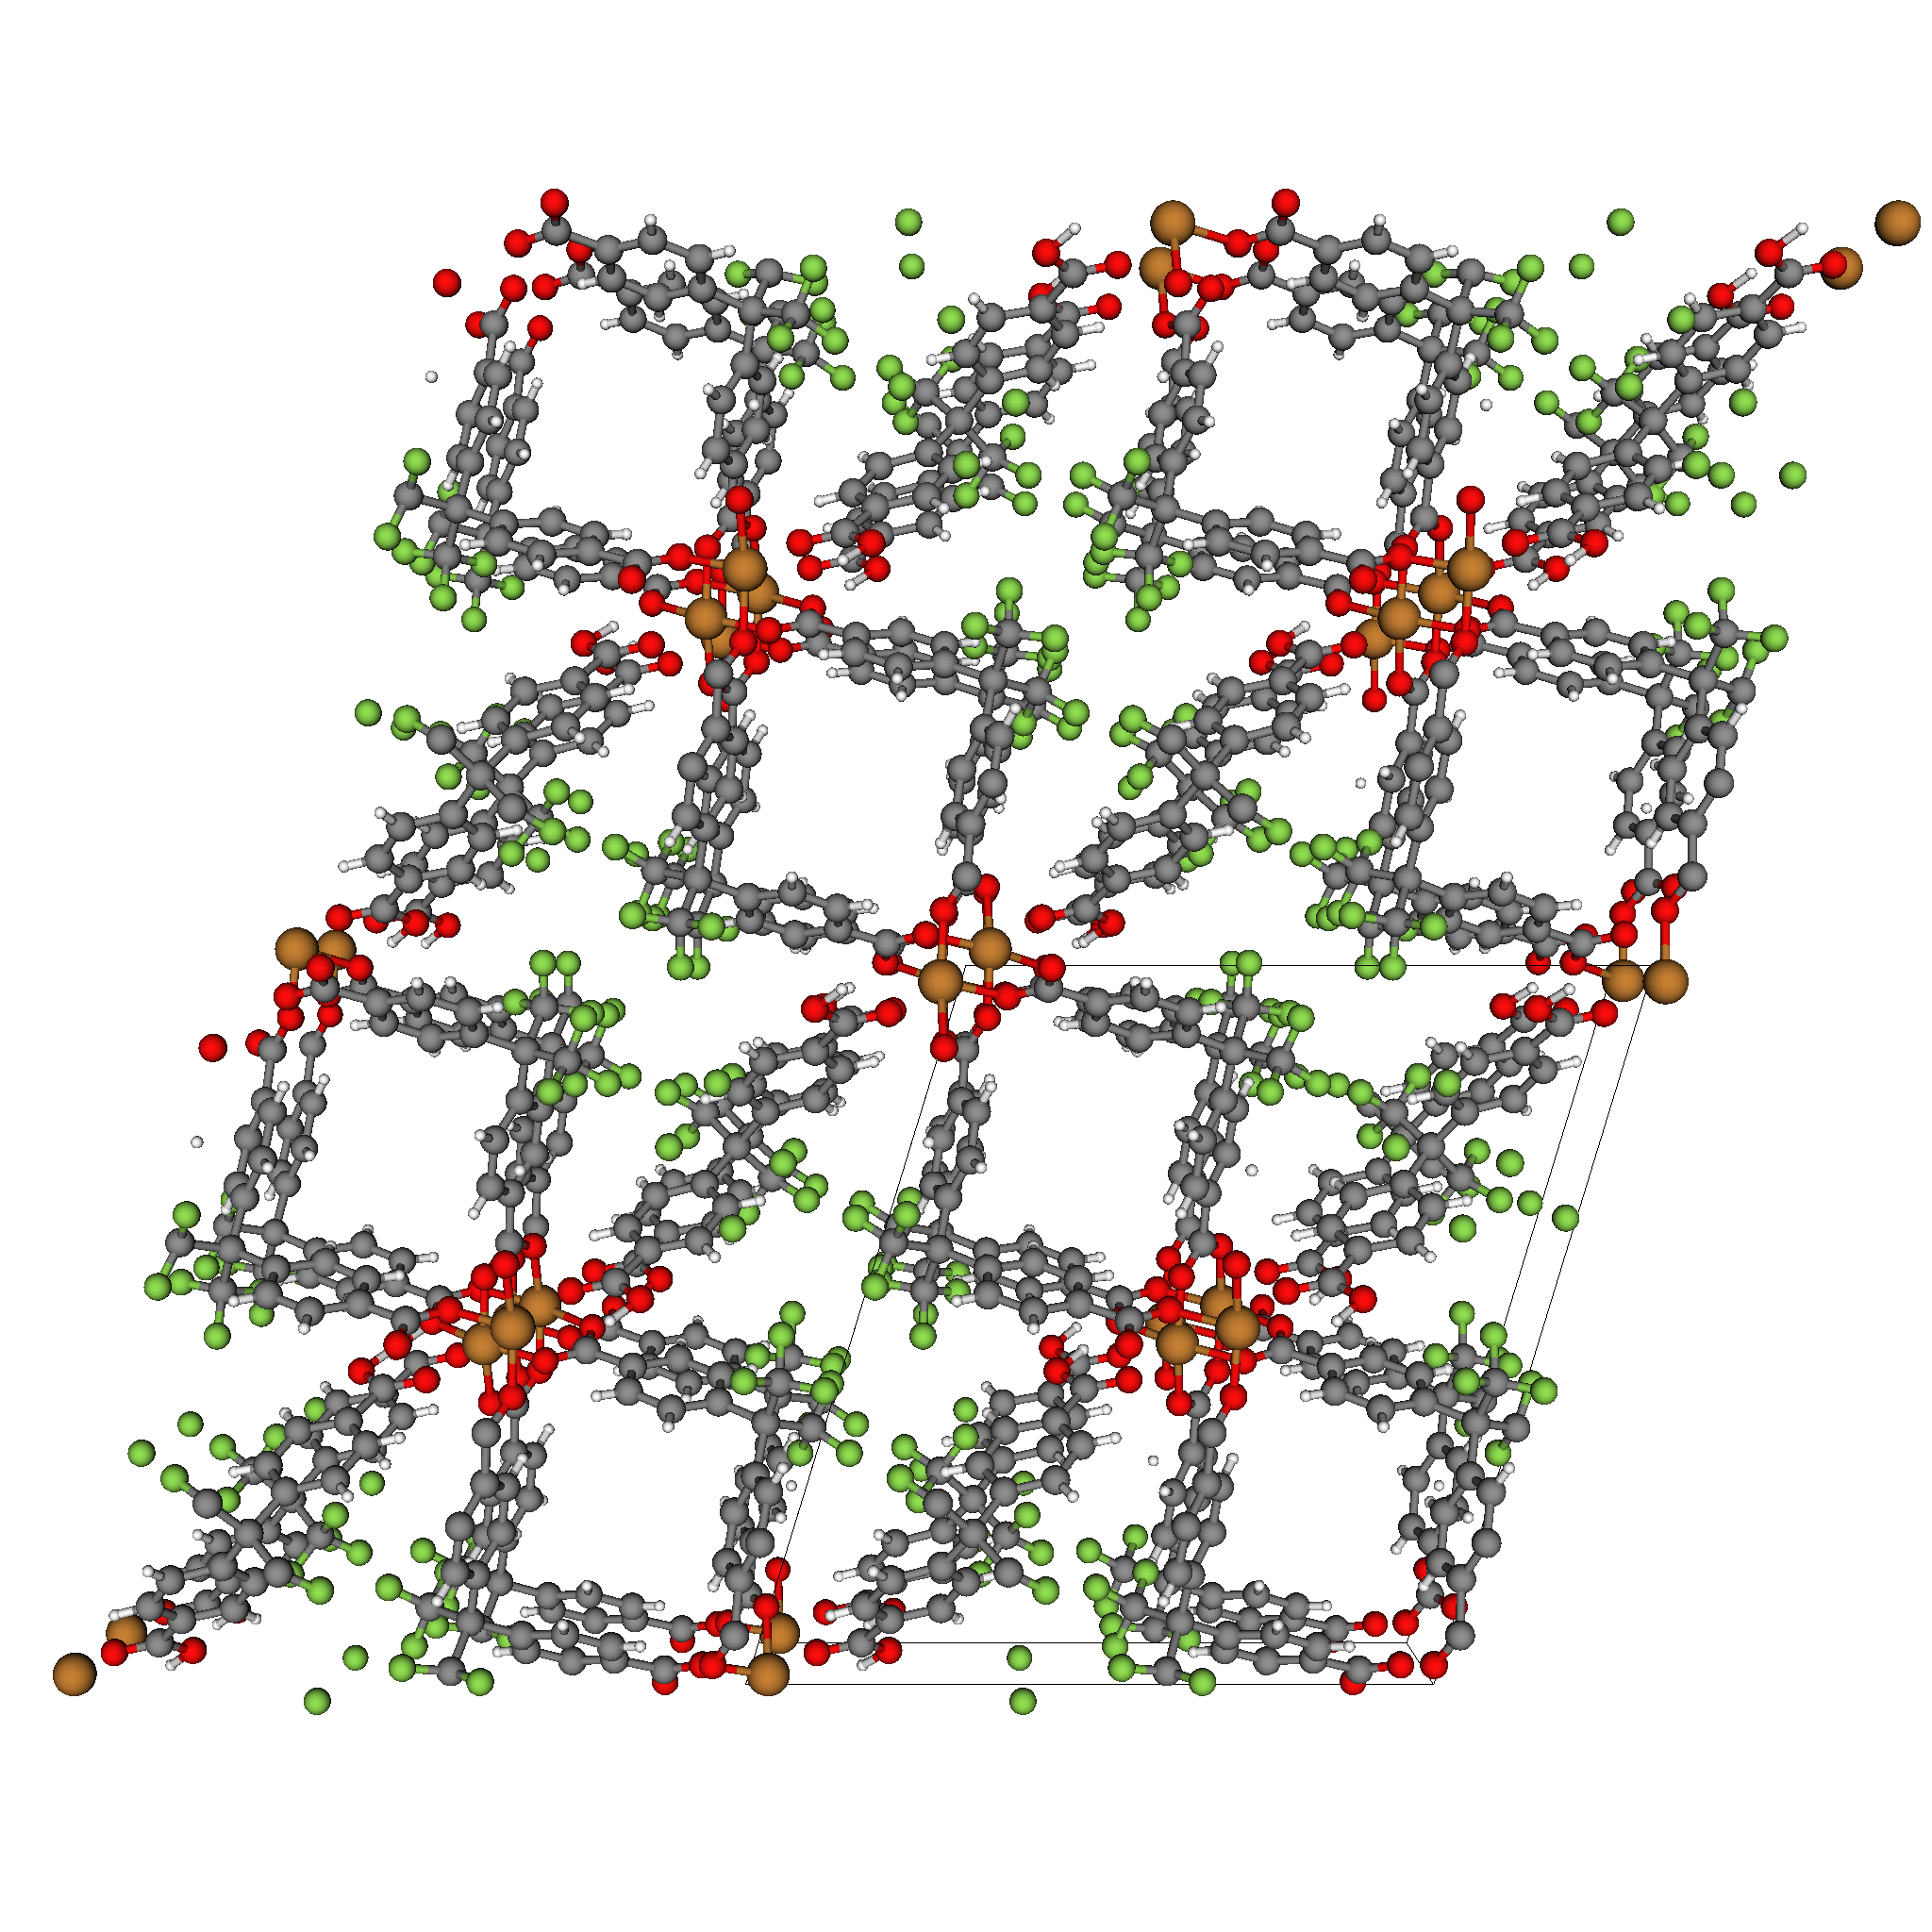
\includegraphics[width=.3\columnwidth]{../xtal_structures/viz/FMOF-Cu.png} \label{fig:FMOF-Cu_xtal} }
       \subfigure[]{\includegraphics[width=.6\columnwidth]{../fits/FMOF-Cu_fit.png} \label{fig:FMOF-Cu_xtal} }
  
       \subfigure[]{\includegraphics[width=.45\columnwidth]{../fits/Xe_low_pressure_fit_FMOF-Cu.png} \label{fig:FMOF-Cu_Xe_KH} }
       \subfigure[]{\includegraphics[width=.45\columnwidth]{../fits/Kr_low_pressure_fit_FMOF-Cu.png} \label{fig:FMOF-Cu_Kr_KH} }
       
       \caption{FMOF-Cu. (a) Crystal structure \cite{FMOF-Cu_structure}.
       (b) Circles show pure-component Xe (blue) and Kr (red) adsorption isotherm data at 297 K from Ref. \cite{FMOF-Cu_XeKr}. 
       Closed symbols are data used to identify the Henry coefficient. The dashed line shows Henry's law with the identified Henry coefficient.
       (c, d) Same as (b) but zoomed into the Henry regime. Identified Henry coefficient is shown in the box.}
    \end{figure}
    
    \clearpage
    
    
    \section{MOF-505}
    
    \begin{figure}[h!]
       \centering
       \subfigure[]{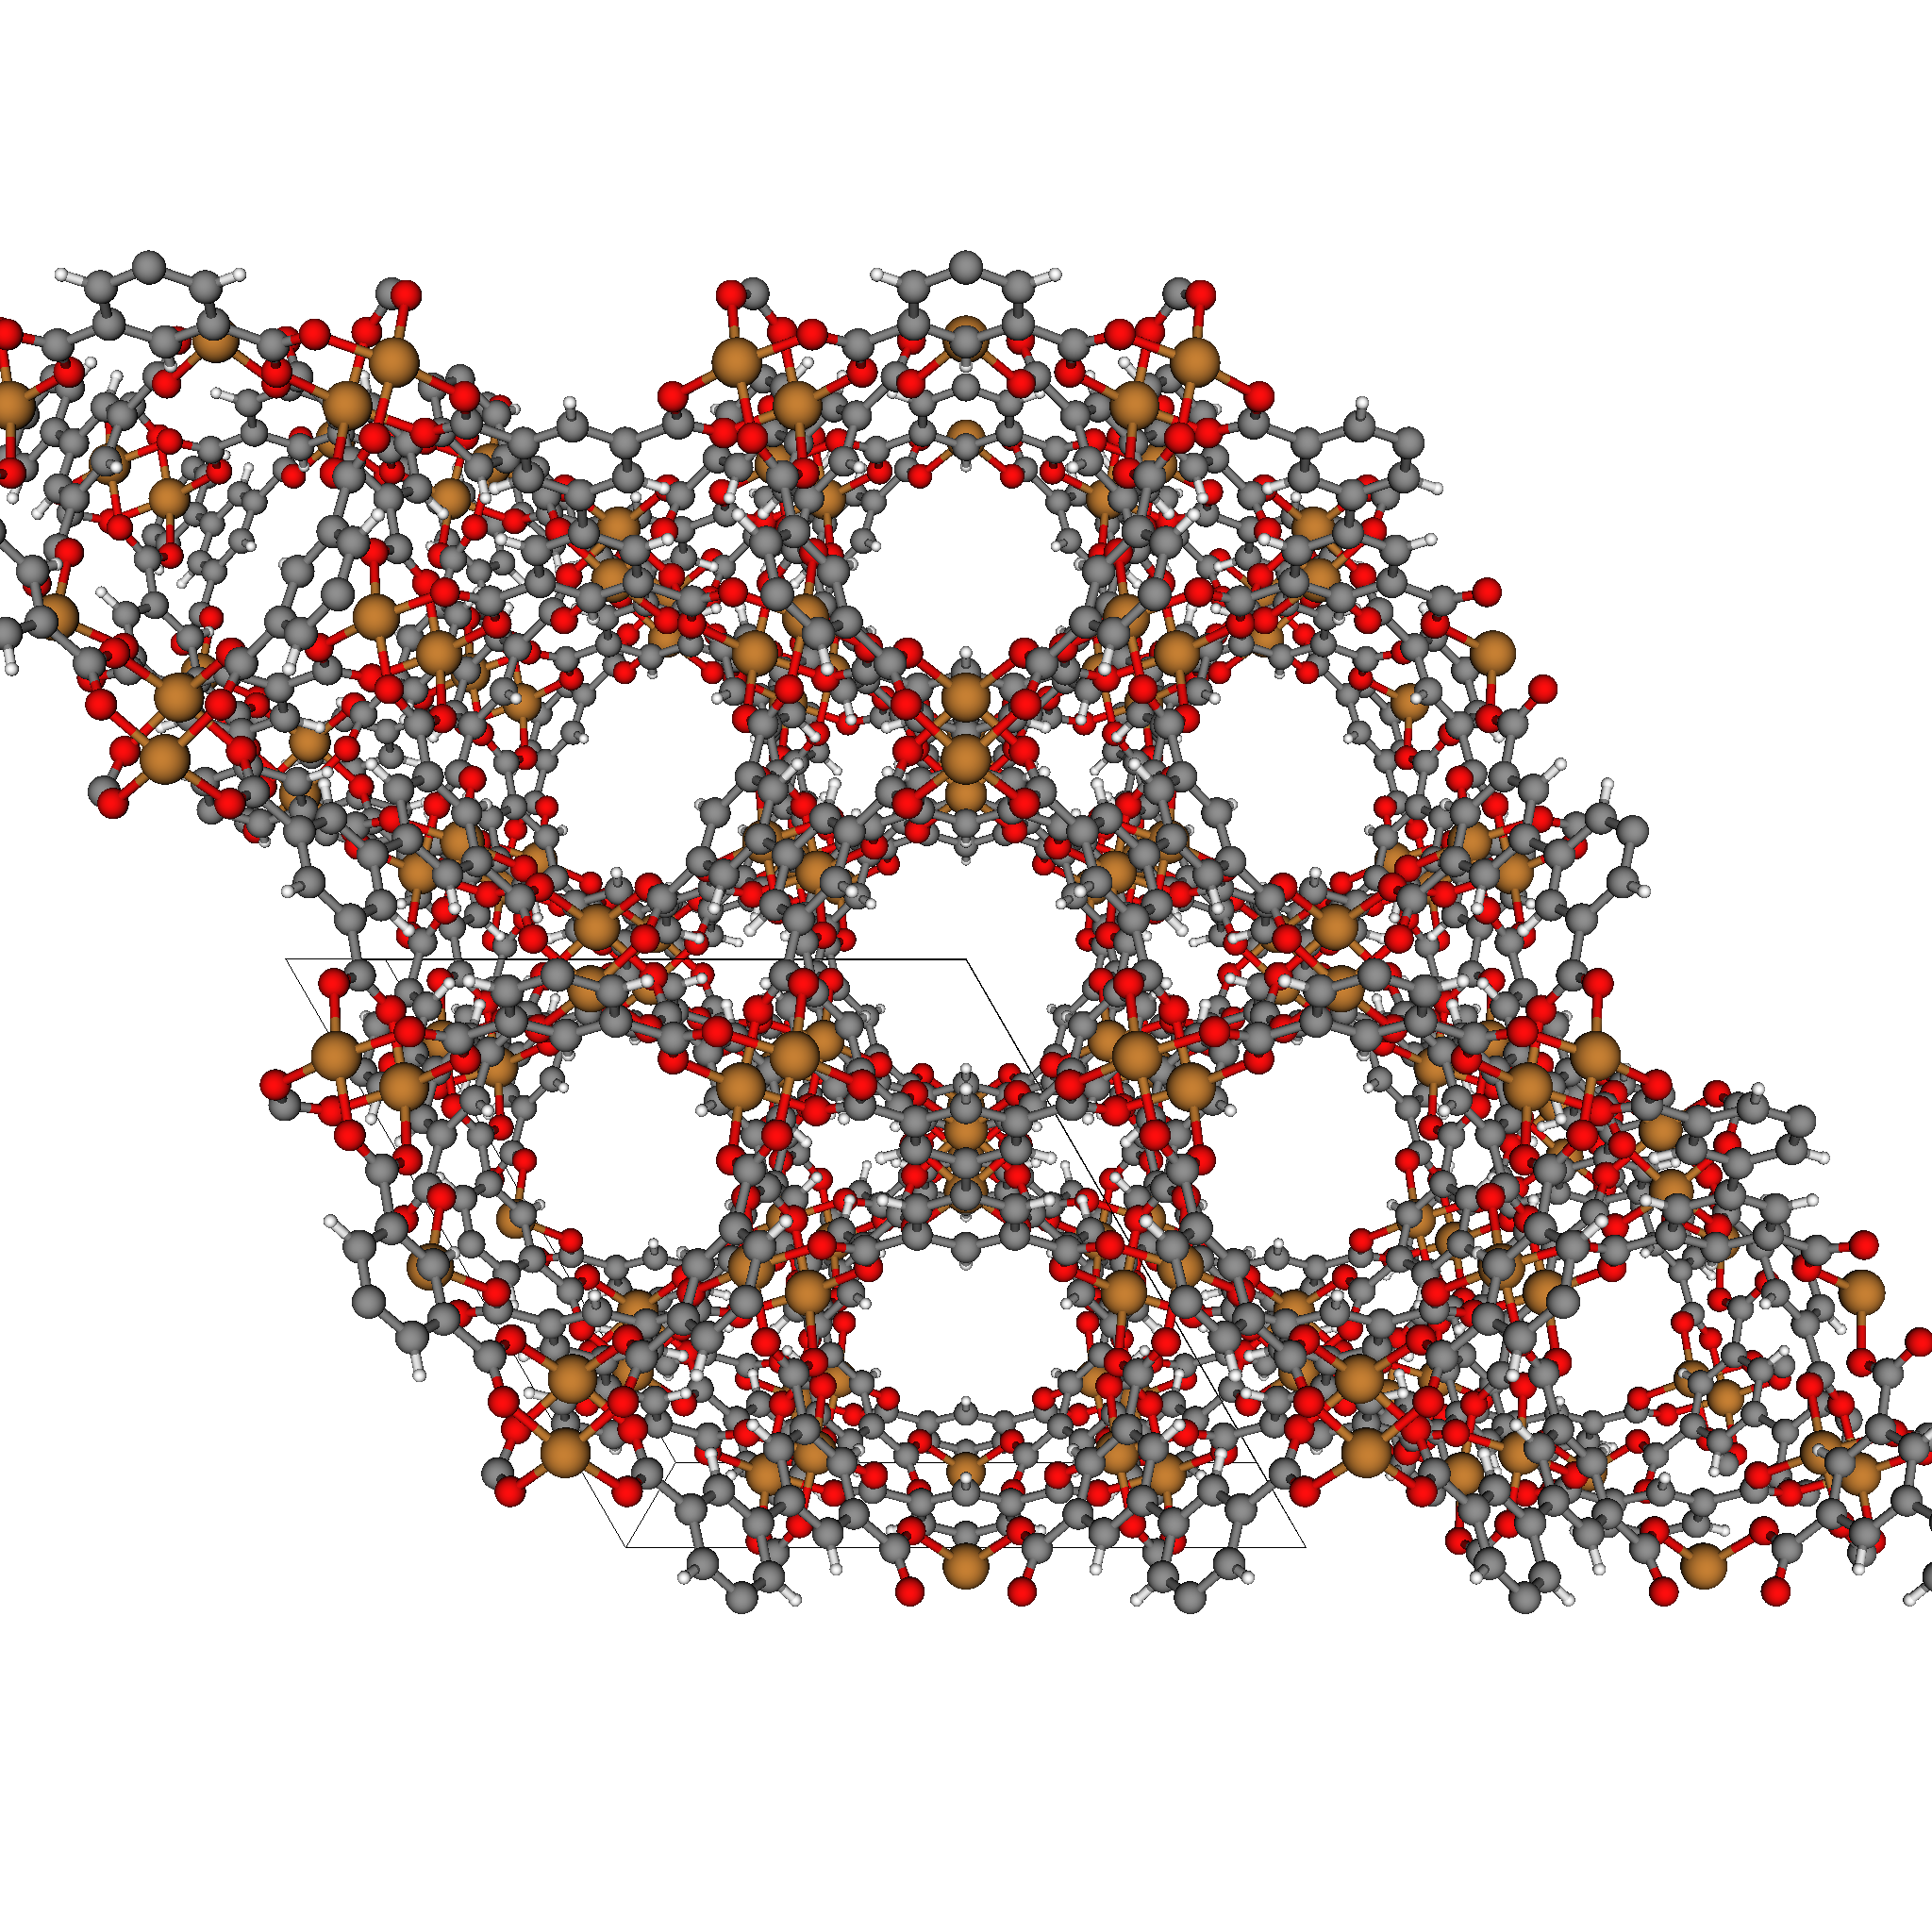
\includegraphics[width=.3\columnwidth]{../xtal_structures/viz/MOF-505.png} \label{fig:MOF-505_xtal} }
       \subfigure[]{\includegraphics[width=.6\columnwidth]{../fits/MOF-505_fit.png} \label{fig:MOF-505_xtal} }
  
       \subfigure[]{\includegraphics[width=.45\columnwidth]{../fits/Xe_low_pressure_fit_MOF-505.png} \label{fig:MOF-505_Xe_KH} }
       \subfigure[]{\includegraphics[width=.45\columnwidth]{../fits/Kr_low_pressure_fit_MOF-505.png} \label{fig:MOF-505_Kr_KH} }
       
       \caption{MOF-505. (a) Crystal structure \cite{MOF-505_structure}.
       (b) Circles show pure-component Xe (blue) and Kr (red) adsorption isotherm data at 292 K from Ref. \cite{MOF-505_XeKr}. 
       Closed symbols are data used to identify the Henry coefficient. The dashed line shows Henry's law with the identified Henry coefficient.
       (c, d) Same as (b) but zoomed into the Henry regime. Identified Henry coefficient is shown in the box.}
    \end{figure}
    
    \clearpage
    
    
    \section{PCN-14}
    
    \begin{figure}[h!]
       \centering
       \subfigure[]{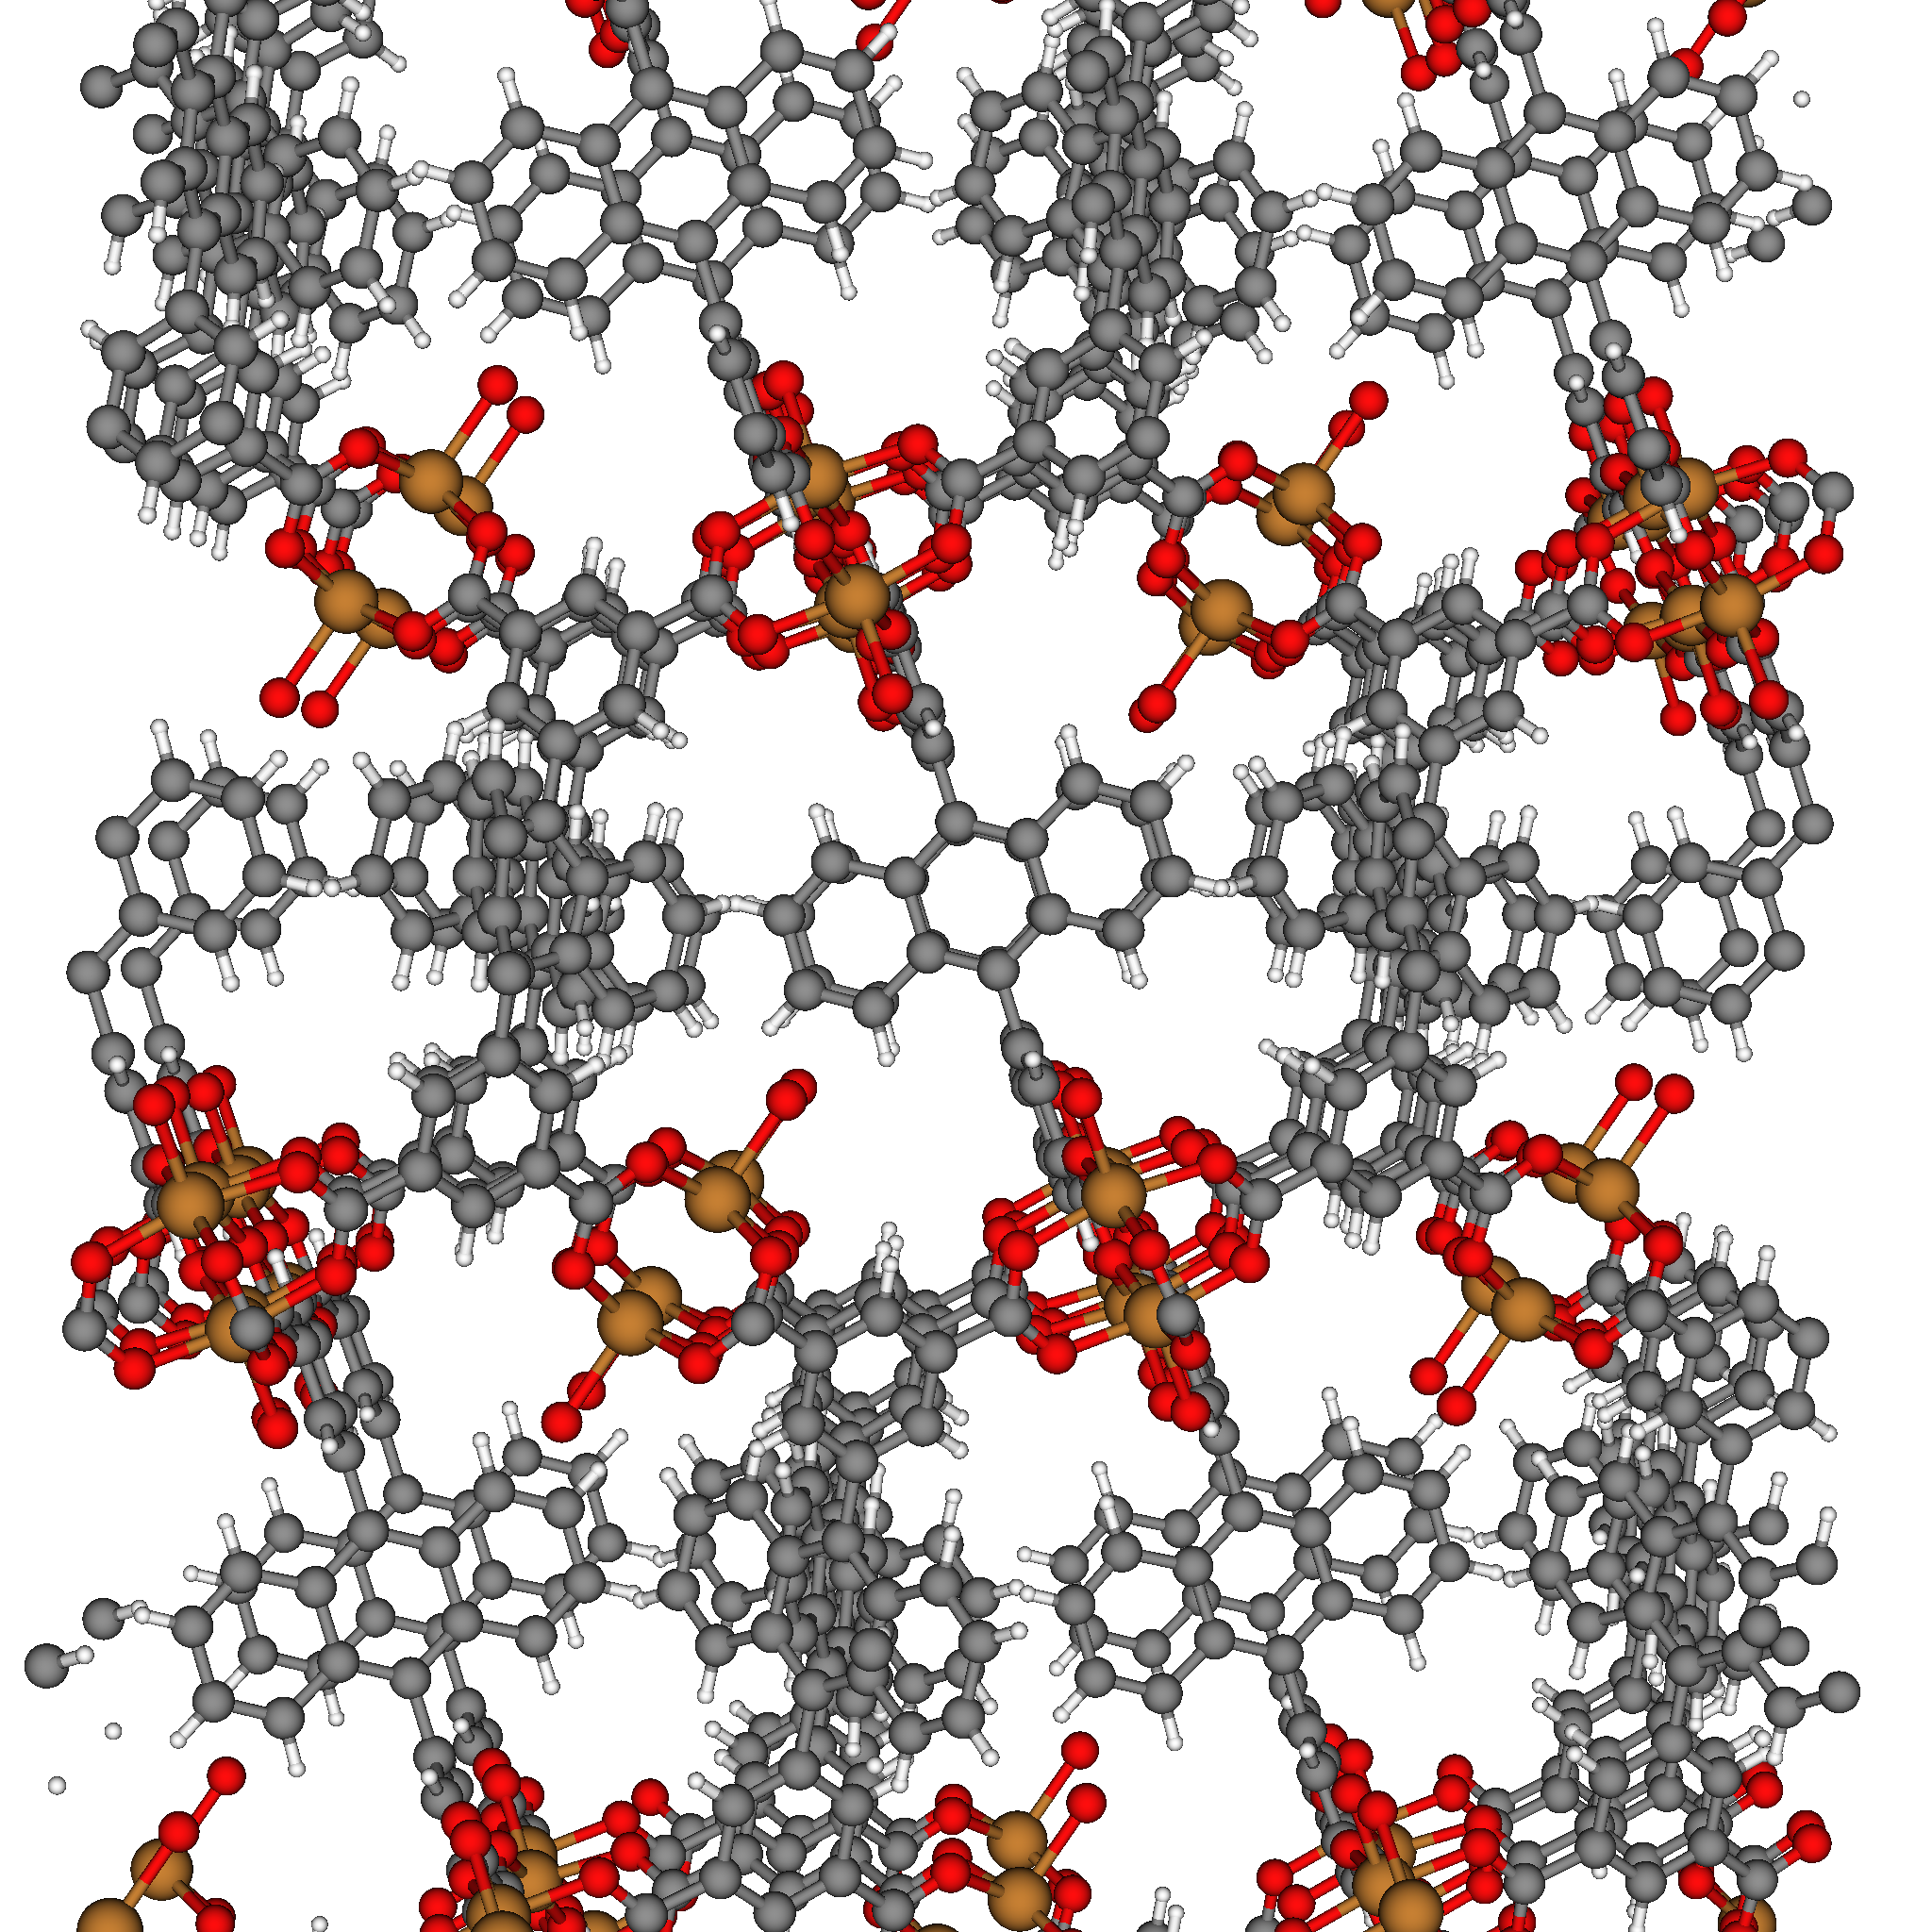
\includegraphics[width=.3\columnwidth]{../xtal_structures/viz/PCN-14.png} \label{fig:PCN-14_xtal} }
       \subfigure[]{\includegraphics[width=.6\columnwidth]{../fits/PCN-14_fit.png} \label{fig:PCN-14_xtal} }
  
       \subfigure[]{\includegraphics[width=.45\columnwidth]{../fits/Xe_low_pressure_fit_PCN-14.png} \label{fig:PCN-14_Xe_KH} }
       \subfigure[]{\includegraphics[width=.45\columnwidth]{../fits/Kr_low_pressure_fit_PCN-14.png} \label{fig:PCN-14_Kr_KH} }
       
       \caption{PCN-14. (a) Crystal structure \cite{PCN-14_structure}.
       (b) Circles show pure-component Xe (blue) and Kr (red) adsorption isotherm data at 292 K from Ref. \cite{PCN-14_XeKr}. 
       Closed symbols are data used to identify the Henry coefficient. The dashed line shows Henry's law with the identified Henry coefficient.
       (c, d) Same as (b) but zoomed into the Henry regime. Identified Henry coefficient is shown in the box.}
    \end{figure}
    
    \clearpage
    
    